\documentclass[parskip=full,11pt,twoside]{scrartcl}

\usepackage[l2tabu,orthodox]{nag}
\usepackage[utf8]{inputenc}

\titlehead{\centering
\includegraphics[width=6cm]{img/logo.pdf}}
\title{Wavelength}
\subtitle{$\bm{\lambda}$-IDE}
\author{Muhammet Guemues, Markus Himmel, Marc Huisinga,\\Philip Klemens, Julia Schmid, Jean-Pierre von der Heydt}

% section numbers in margins:
\renewcommand\sectionlinesformat[4]{\makebox[0pt][r]{#3}#4}

% header & footer
\usepackage{scrlayer-scrpage}
\lofoot{\today}
\refoot{\today}
\pagestyle{scrheadings}

\usepackage[sfdefault,light]{roboto}
\usepackage[T1]{fontenc}
\usepackage[ngerman]{babel}
\usepackage{datetime2}
\usepackage[hidelinks]{hyperref}
\usepackage[nameinlink]{cleveref}
\crefname{figure}{Abb.}{Abb.}
\usepackage[section]{placeins}
\usepackage{xcolor}
\usepackage{graphicx}
\hypersetup{
	pdftitle={Pflichtenheft},
	bookmarks=true,
}
\usepackage{csquotes}

\usepackage{amsmath}
\usepackage{bm}
\usepackage{mathtools}
\usepackage{amssymb}
\usepackage{float}
\usepackage{subcaption}

\usepackage{glossaries}
\GlsSetQuote{+}
%
\usepackage{pkg/pflichtenheft}

\MakeOuterQuote{"}

\makeglossaries

\newglossaryentry{lk}
{ 
	name=$\lambda$-Kalkül,
	description={Der $\lambda$-Kalkül ist eine formale Sprache, die, basierend auf Funktionsdefinitionen, eine systematische Untersuchung von Funktionen zulässt}
}
\newglossaryentry{lapp}
{ 
	name=$\lambda$-Applikation,
	plural=$\lambda$-Applikationen,
	description={Applikationen stellen die Anwendung eines \gls{lt}s auf einen weiteren \gls{lt} dar. Sie haben im Allgemeinen die Form: \emph{<\gls{lt}1> <\gls{lt}2>}, wobei die spitzen Klammern hier nur der Übersicht wegen eingefügt wurden und im eigentlichen 			    Ausdruck nicht vorkommen}
}
\newglossaryentry{labs}
{ 
	name=$\lambda$-Abstraktion,
	plural=$\lambda$-Abstraktionen,
	description={Abstraktionen stellen eine Funktionsdefinition einer Funktion in einer Variablen dar. Abstraktionen haben die Form \emph{$\lambda$} <\gls{var}>.<\gls{lt}>, wobei die Ausdrücke in den spitzen Klammern inklusive der spitzen Klammern durch die entsprechenden Objekte zu ersetzen sind}
}
\newglossaryentry{lt}
{
	name=$\lambda$-Term,
	plural=$\lambda$-Terme,
	description={Terme im \gls{lk} sind entweder \emph{\glspl{lapp}} oder \emph{\glspl{labs}} oder \emph{\glspl{var}}}
}
\newglossaryentry{lit}
{
	name=Literal,
	plural=Literale,
	description={Zeichenfolge, die Werte von Basistypen repräsentiert. Im vorliegenden
		Dokument werden nur Literale für natürliche Zahlen in Dezimaldarstellung betrachtet}
}
\newglossaryentry{var}
{ 
	name=Variable,
	plural=Variablen,
	description={Variablen sind Platzhalter für konkrete Werte. Als Variablen zugelassen sind beliebige Zeichen und Zeichenkombinationen ohne die folgenden Zeichen:
	\begin{tabular} {| l | c | c | c | c | c | r |}
	\hline
	 $\lambda$ & . & \textbackslash & : & = & ( & ) \\
	 \hline
	\end{tabular}
	}
}
\newglossaryentry{alpha} 
{
	name=$\alpha$-Konversion,
	description={Die $\alpha$-Konversion entspricht einer Variablenumbenennung in einer \gls{lapp}. \underline{Beispiel:} Umbenennung von x in y: $\lambda x.T \stackrel{\alpha}{\Rightarrow} \lambda y.T[y/x]$}
}
\newglossaryentry{beta}
{
	name=$\beta$-Reduktion,
	plural=$\beta$-Reduktionen,
	description={Die $\beta$-Reduktion entspricht einer Funktionsauswertung. Sie ist nur auf \glspl{redex} anwendbar.
			Sollten durch die Auswertung freie Variablen gebunden werden, so müssen diese vorher durch \gls{alpha} in ungenutzte Variablen umbenannt werden.
	 		Formal gilt für eine Variable $V$ und \glspl{lt} $T_1$ und $T_2$ die \gls{subs}: $(\lambda V.T_1) T_2 \stackrel{\beta}{\Rightarrow} T_1[T_2/V]$}
}
\newglossaryentry{redex} 
{
	name=Redex,
	plural=Redexe,
	description={Redexe (Reducible Expressions) sind Ausdrücke der Form \emph{($\lambda$.\gls{lt}1) \gls{lt}2}}
}
\newglossaryentry{fv} 
{
	name=freie Variable,
	plural=freie Variablen,
	description={Eine Variable in einem \gls{lt} heißt \emph{frei}, wenn sie kein Parameter einer \gls{labs} ist}
}
\newglossaryentry{gv} 
{
	name=gebundene Variable,
	plural=gebundene Variablen,
	description={Eine Variable in einem \gls{lt} heißt \emph{gebunden}, wenn sie Parameter einer \gls{labs} ist}
}
\newglossaryentry{subs}
{
	name=Substitution,
	plural=Substitutionen,
	description={Bei einer Substitution einer \glspl{var} $y$ in einer \gls{labs} $\lambda x.T_1$, wobei $T_1$ ein \gls{lt} ist,  werden alle freien Vorkommen von $x$ in $T_1$ durch $y$ ersetzt und der Parameter in y umbenannt. 
			In Formeln: $\lambda x.T_1 \stackrel{\text{Substitution mit $y$}}{\Longrightarrow}\lambda y.[T_1/y]$}
}
\newglossaryentry{aws}
{
	name=Auswertungsstrategie,
	plural=Auswertungsstrategien,
	description={Eine Auswertungsstrategie ist ein Algorithmus, der bestimmt, wie ein \gls{lt} ausgewertet wird. Dabei kann es vorkommen, dass eine Auswertungsstrategie bei der Auswertung eines \gls{lt} in eine Endlosschleife gerät, während eine andere 				Strategie terminiert}
}
\newglossaryentry{nr}
{
	name=normale Reduktionsordnung,
	description={Die normale Reduktionsordnung ist eine \gls{aws}, bei der immer der linkeste äußerste \gls{redex} zuerst $\beta$-reduziert wird}
}
\newglossaryentry{cbn}
{
	name=Call by Name,
	description={Call by Name ist eine \gls{aws}, bei der der linkeste äußerste \gls{redex}, der nicht von einem $\lambda$ umgeben ist, zuerst $\beta$-reduziert wird}
}
\newglossaryentry{cbv}
{
	name=Call by Value,
	description={Call by Value ist eine \gls{aws}, bei der der linkeste äußerste \gls{redex}, der nicht von einem $\lambda$ umgeben ist und dessen Argument ein konkreter Wert ist, zuerst $\beta$-reduziert wird}
}
\newglossaryentry{yc} 
{
	name=Y-Kombinator,
	description={Formal dient der Y-Kombinator dazu, \gls{rec} zu ermöglichen. Er ist definiert als: $Y \coloneqq \lambda f.(\lambda x.f(x\,x))(\lambda x.f(x\,x))$}
}	
\newglossaryentry{rec}
{
	name=Rekursion,
	description={Eine Funktion heißt rekursiv, wenn sie sich selbst aufruft. Der Aufruf wird dann als Rekursion bezeichnet}
}
\newglossaryentry{brow}
{
	name=kompatibler Browser,
	plural=kompatible Browser,
	description={Als kompatible Browser gelten die folgenden:
	\begin{itemize}
	\item Microsoft Edge ab Version 41.16299.15.0
	\item Mozilla Firefox ab Version 57.0
	\item Google Chrome ab Version 62.0.3202
	\end{itemize}}
}

\newglossaryentry{ao}
{
	name=Applicative Order,
	description={Eine \gls{aws}, bei der der rechteste innerste Redex zuerst $\beta$-reduziert wird}
}
\newglossaryentry{mfe}
{
	name=Mehrfacheinrückung,
	plural=Mehrfacheinrückungen,
	description={Alle markierten Zeilen werden eingerückt}
}
\newglossaryentry{st}
{
	name=Smart Tab,
	plural=Smart Tabs,
	description={Beim Erstellen einer neuen Zeile wird die neue Zeile genauso eingerückt wie die Zeile von der die neue Zeile aus erzeugt wird}
}

\newglossaryentry{vls}
{
	name={vereinfachte $\lambda$-Syntax},
	description={Variante der herkömmlichen Syntax des \glslink{lk}{$\lambda$-Kalküls},
	bei der das $\lambda$-Symbol durch ein \texttt{\textbackslash}-Symbol ersetzt wird
	und natürliche Zahlen in Dezimaldarstellung anstelle von \glspl{cn} verwendet werden
	können.
	Ferner besteht die Möglichkeit zur \gls{nb}. Ein korrekter Term in der vereinfachten
	$\lambda$-Syntax besteht aus einer beliebigen Zahl von Namensbindungen gefolgt von
	genau einem freistehenden \gls{lt}}
}

\newglossaryentry{cn}
{
	name=Church-Zahl,
	plural=Church-Zahlen,
	description={Gängige Umsetzung der natürlichen Zahlen inklusive der Null im \gls{lk}. $n\in\mathbb{N}_0$ wird dargestellt als $\lambda f.\lambda x. \underbrace{f\cdots f}_{\text{$n$ mal}} x$}
}

\newglossaryentry{cmpltapp}
{
	name=Komplettauswertung,
	description={Wiederholte \gls{beta} auf einem \gls{lt} basierend auf einer gegebenen \gls{aws}. 
	Muss nicht zwingend terminieren}
}

\newglossaryentry{nrmlform}
{
	name={$\beta$-Normalform},
	description={Ein \gls{lt} ist in $\beta$-Normalform, wenn keine \gls{beta} mehr anwendbar ist}
}
\newglossaryentry{nb}
{
	name=Namensbindung,
	description={Einem \gls{lt} kann ein Name zugewiesen werden. 
		Danach steht dieser Name als Ersatz für den \gls{lt}.
		Die Zuweisung hat die Form: <Name> $\coloneqq$ <\gls{lt}>, wobei die spitzen Klammern hier nur
		der Übersicht wegen eingefügt wurden und im eigentlichen Ausdruck nicht vorkommen.
		Auf der rechten Seite des Gleichheitszeichen darf der Name selbst nicht verwendet werden.
		Als Name zugelassen sind alle Zeichen und Zeichenfolgen ohne die folgenden Zeichen: 
		\begin{tabular}{| l | c | c | c | c | c | r |}
			\hline
				$\lambda$ & . & = & : & \textbackslash & ( & )\\
			\hline
		\end{tabular}}
}
\newglossaryentry{ex}
{
	name=Übungsaufgabe,
	plural=Übungsaufgaben,
	description={Eine Übungsaufgabe besteht aus einer Beschreibung und eventuell einem Stück Code.
	 Beim Laden der Übungsaufgabe wird die Beschreibung in das Aufgabenfeld eingefügt.
	 Der Code wird ins Eingabefeld eingefügt}
}
\newglossaryentry{std}
{
	name=Standardeinstellung,
	plural=Standardeinstellungen,
	description={Standardmäßig sind folgende Einstellungen ausgewählt:
	 \begin{itemize}
	 \item Modus: Eingabemodus (vgl. \cref{fig:state})
	 \item \gls{aws}: \gls{nr} (vgl. \cref{fig:outputOptions})
	 \item Ausgabeformat: Unicode (vgl. \cref{fig:outputOptions})
	 \item Ausgabeumfang: Result only (vgl. \cref{fig:outputOptions})
	 \end{itemize}}
}

% Syntax:
%\newglossaryentry{label}
%{
%	name=Name,
%	plural=Namen,
%	description={Beschreibung}
%}

% Verwendung der Glossareinträge:
% Normalerweise \gls{label}
% Am Anfang des Satzes \Gls{label}
% Bei Plural: \glspl{label}
% Bei Plural am Anfang des Satzes: \Glspl{label}
% Falls nichts davon passt: \glslink{label}{Anderer Text}

%%% Ende Glossareinträge

\begin{document}
\maketitle
\thispagestyle{empty}
\pagebreak

\tableofcontents
\pagebreak

\section{Einleitung}
Ziel dieses Projektes ist die Bereitstellung einer Online-Entwicklungsumgebung für den \gls{lk}. 
Sie kann direkt über einen \glslink{brow}{kompatiblen Browser} verwendet werden.
Die Entwicklungsumgebung wird für die Lehre entworfen: 
Sie kann von Dozenten zur Demonstration eingesetzt werden, ebenso kann sie von Studenten zum Lernen verwendet werden.
Mit der Anwendung können \glspl{lt} eingegeben und entsprechend einer \gls{aws} ausgewertet werden.
Dabei kann die Auswertung auch Schritt für Schritt verfolgt werden.
Der Lernprozess wird durch ein System von Übungsaufgaben unterstützt.

\pagebreak
\section{Kriterien}
% Diese Section sollte kurz und knapp "für Manager" sein
% und auf eine Seite passen.

\subsection{Muss}

\criterium{Eingabe von \glslink{lt}{$\lambda$-Termen}}{crt:input}
\glspl{lt} können in Form der \glslink{vls}{vereinfachten $\lambda$-Syntax}
mit der Tastatur in die Software eingegeben werden.

\criterium{Auswertung von \glslink{lt}{$\lambda$-Termen}}{crt:reduce}
Eingegebene \glspl{lt} können, sofern möglich, mit Hilfe der \glslink{nr}{Normal-Reduktionsordnung} vollständig
reduziert werden. Die so bestimmte Normalform kann in \glslink{vls}{vereinfachter $\lambda$-Syntax}
dargestellt werden.

\criterium{Fehlermeldung bei invalider Eingabe}{crt:error}
Beim Versuch, einen syntaktisch inkorrekten \gls{lt} reduzieren zu lassen, wird eine
Fehlermeldung ausgegeben.

\criterium{Abbruch der Reduktion}{crt:cancel}
Der Benutzer kann die Reduktion eines \glslink{lt}{$\lambda$-Terms} abbrechen.

% Syntax:
% \criterium{Überschrift des Kriteriums}{crt:label}
% Beschreibung des Kriteriums

\subsection{Kann}

\criteriumOptional{Weitere \glspl{aws}}{crt:awsstrats}
Die Anwendung kann neben der \glslink{nr}{Normal-Reduktionsordnung} auch \gls{cbn}, \gls{cbv}
und \gls{ao} als \gls{aws} verwenden.

\criteriumOptional{Exportformate}{crt:output}
Die eingegebenen und reduzierten \glspl{lt} können neben der \glslink{vls}{vereinfachten $\lambda$-Syntax}
auch als Unicode-Text, \LaTeX-Quellcode, Haskell-Quellcode und Lisp-Quellcode formatiert und exportiert
werden.

\criteriumOptional{Ausgabeformate}{crt:display}
Die eingegebenen und reduzierten \glspl{lt} können innerhalb der Applikation in Unicode-Ausgabe und als Syntaxbaum
ausgegeben werden.

\criteriumOptional{Erweiterte Fehlerdiagnostik}{crt:diag}
Im Falle syntaktischer Fehler werden dem Nutzer die genaue Position des Fehlers, die
Art des Fehlers sowie Behebungsmöglichkeiten angezeigt und die relevante Stelle im
Editor hervorgehoben.

\criteriumOptional{Intelligenter Editor}{crt:editor}
Der Editor zur Eingabe der \glspl{lt} unterstützt Standard-Editor-Funktionen,
\glspl{mfe} und \glspl{st}.

\criteriumOptional{Standardbibliothek}{crt:lib}
Es existiert eine Standardbibliothek, die Funktionen für den Umgang mit natürlichen
Zahlen, Listen, Tupeln, Booleans und dem \gls{yc} bereitstellt.

\criteriumOptional{Übungsaufgaben}{crt:ex}
Das Programm enthält ein Übungsaufgaben-System, welches neben Aufgaben in aufsteigendem
Schwierigkeitsgrad auch Einführungen und automatisierte Tests für die Lösungen des Nutzers
enthält.

\criteriumOptional{Ausgabe von Teilschritten}{crt:partial}
Die zum Erreichen der Normalform notwendigen Reduktionsschritte gemäß der ausgewählten
\gls{aws} können im ausgewählten Ausgabeformat ausgegeben werden. Hierbei
können entweder alle Teilschritte, die ersten und letzten Teilschritte, oder
einzelne Teilschritte in periodischen Abständen angezeigt werden.

\criteriumOptional{Schritt-für-Schritt-Modus}{crt:steps}
Es existiert ein Schritt-für-Schritt-Modus, welcher entweder direkt von der Eingabe
oder durch Pausieren einer laufenden Reduktion erreicht werden kann.
Durch Klicken kann ein bestimmter Teilausdruck ausgewertet werden oder die ausgewählte
\gls{aws} einen einzelnen Schritt machen. Diese Auswertungsschritte können rückgängig
gemacht werden.

\criteriumOptional{Permalinks}{crt:perma}
Es kann ein Link generiert werden, der beim Aufrufen den gesamten Zustand
der Sitzung wiederherstellt.

\criteriumOptional{Komfortabler $\lambda$-Code}{crt:comfcode}
Einem \gls{lt} kann ein Name zugewiesen werden. Dieser kann anstelle des Terms
verwendet werden. Außerdem können Kommentare geschrieben werden, die bei der
Auswertung nicht beachtet werden.
% Syntax:
% \criteriumOptional{Überschrift des Kriteriums}{crt:label}
% Beschreibung des Kriteriums


\subsection{Abgrenzung}

% Syntax:
% \criteriumNot{Überschrift der Abgrenzung}{ctr:label}
\criteriumNot{Nutzung über Mobilgeräte}{crt:mobile}
Die Anwendung muss nicht auf mobilen Endgeräten einsetzbar sein.

\criteriumNot{Lokalisierung}{crt:lokal}
Die Anwendung soll nur in englischer Sprache verfügbar sein.

\pagebreak

\section{Funktionale Anforderungen}

\functionality{Editor}{fnc:ed}
\fulfills{crt:input}
\fulfills{crt:editor}
Nutzer können beliebigen Text in einem Eingabefeld eingeben. 
Das Eingabefeld verfügt über Standard-Textfeld-Funktionalitäten mit dazugehörigen gängigen Tastenkombinationen:
\begin{itemize}
	\item Editieren, Markieren und Navigieren von Text im Eingabefeld
	\item Kopieren, Ausschneiden und Einfügen
	\item Undo und Redo
\end{itemize}
Außerdem verfügt das Eingabefeld über \gls{st}s und \gls{mfe}.
Bei der Eingabe einer öffnenden Klammer wird auch direkt die schließende Klammer hinter der öffnenden Klammer eingefügt.
Wird der Editor-Cursor vor oder hinter eine Klammer bewegt, so wird die zugehörige schließende Klammer angezeigt.
Neben dem Eingabefeld werden Zeilennummern angezeigt.

\functionality{\gls{cmpltapp}}{fnc:completereduce}
\fulfills{crt:reduce}
Der Nutzer hat die Möglichkeit, auf einen eingegebenen \gls{lt} automatisch \glspl{beta} anwenden zu lassen. 
Die hierzu verwendete \gls{cmpltapp} wird durch das Drücken des Start-Knopfes (\cref{fig:actionButtons}) gestartet.
Ist die Eingabe syntaktisch falsch, so wird eine Fehlermeldung ausgegeben und die Komplettauswertung verlassen.

Es werden die Knöpfe zum Laden von Bibliotheken und Aufgaben sowie der Schritt-für-Schritt-Knopf deaktiviert.
Außerdem werden das Eingabefeld, das Ausgabeformats-, das \gls{aws}-Dropdown-Menü und das Ausgabeumfangs-Dropdown-Menü deaktiviert.
Der Start-Knopf wird zu einem Pause-Knopf.

Die Reihenfolge der \glspl{beta} wird durch die derzeit aktive \gls{aws} bestimmt. Die Ausgabe wird durch das derzeit aktive Ausgabeformat (\cref{fig:outputOptions}) und den derzeitig aktiven Ausgabeumfang bestimmt.

Die Komplettauswertung übernimmt die automatische Auswertung, bis die derzeit aktive \gls{aws} keine \gls{beta} mehr vorgibt.
Wenn der \gls{lt} keine \gls{nrmlform} besitzt oder die \gls{aws} diese nicht findet, terminiert die \gls{cmpltapp} nicht.

Wird der Pause-Knopf (siehe \cref{fig:actionButtons}) betätigt, so wechselt die Ausgabe in den Schritt-für-Schritt-Modus und das \gls{aws}-Dropdown-Menü wird wieder aktiviert.

\functionality{Live-Updates der \gls{cmpltapp}}{fnc:live}
\fulfills{crt:partial}
Solange die \gls{cmpltapp} nicht terminiert, wird im Ausgabefeld der derzeitige Ergebnisstand im gewählten Ausgabeumfang ausgegeben. 
Insbesondere bei einer Auswahl des Ausgabeumfangs von "Full" oder "Periodically" werden dem Nutzer regelmäßig die derzeit berechneten \gls{lt} ausgegeben.

%TODO extra funktionale anforderungen für die farbliche markierung von Unicode und Bäumen?
\functionality{Unicode-Ausgabe}{fnc:unicode}
\fulfills{crt:display}
Der Nutzer hat die Möglichkeit, sich Auswertungen von \gls{lt}en in Unicode ausgeben zu lassen. Die Ausgabe wird im Ausgabefeld ausgegeben.\\
Jeder neu ausgegebene Auswertungsschritt wird in einer neuen Zeile ausgegeben. 
Dabei wird am Anfang der Zeile kenntlich gemacht, ob es sich um eine \gls{alpha} oder \gls{beta} handelt (siehe \cref{fig:unicode}).
Wird der Mauszeiger in der letzten Zeile über eine Klammer bewegt, so wird die Klammer und die dazugehörige öffnende oder schließende Klammer markiert.

\functionality{Syntaxbaum-Ausgabe}{fnc:tree}
\fulfills{crt:display}
Der Nutzer hat die Möglichkeit, sich Auswertungen von \gls{lt}en als Syntaxbaum ausgeben zu lassen. Die Ausgabe wird im Ausgabefeld ausgegeben (siehe \cref{fig:tree}).\\
Jeder neu ausgegebene Auswertungsschritt wird als neuer Baum unter dem letzten Auswertungsschritt ausgegeben. Hierbei wird ein \gls{lt} in folgender Weise in einen Baum übersetzt:
\begin{itemize}
	\item \gls{lapp}en werden als Elternknoten mit dem Namen "App" dargestellt. 
	Der erste und zweite \gls{lt} der \gls{lapp} werden als Kindknoten angefügt (\cref{fig:ltAppTreeB}).
	\item \gls{labs}en mit der \gls{var} $x$ werden als Elternknoten mit dem Namen "$\lambda x$" dargestellt. 
	Der Elternknoten besitzt einen Kindknoten, welcher den \gls{lt} der \gls{labs} enthält.
	\item Sollte ein Kindknoten des Baums wieder eine \gls{lapp} oder eine \gls{labs} enthalten, wird dieser Knoten wieder als Eltern und Kindknoten dargestellt (\cref{fig:ltAppTreeA}).
\end{itemize}

\functionality{Auswahl des Ausgabeformats}{fnc:display}
\fulfills{crt:display}
Der Nutzer kann das derzeitig aktive Ausgabeformat über ein Dropdown-Menü auswählen (\cref{fig:outputOptions}).
Das Ausgabeformat entscheidet über die Visualisierung im Ausgabefeld. Das Ausgabeformat hat jedoch keine Auswirkung auf das Exportieren von Ergebnissen.\\
Standardmäßig ist die Unicode-Ausgabe ausgewählt.
Der Nutzer kann das Ausgabeformat nur im Eingabemodus ändern (vgl. \cref{fig:state}).
Das bedeutet insbesondere, dass der Nutzer das Ausgabeformat nicht während einer laufenden Auswertung ändern kann.

\functionality{Auswahl einer \gls{aws}}{fnc:awsstrats}
\fulfills{crt:awsstrats}
Der Nutzer kann die derzeitig aktive \gls{aws} über ein Dropdown-Menü auswählen (\cref{fig:awsOptions})).\\
Die folgenden \gls{aws} können gewählt werden:
\begin{itemize}
	\item Normale-Reduktionsordnung
	\item Call by Name
	\item Call by Value
	\item Applicative Order
\end{itemize}
Die \gls{aws} bestimmt die Reihenfolge von automatischen \glspl{beta} und damit die Markierung des nächsten zu reduzierenden \gls{lt}s im Ausgabefeld (\cref{fig:unicode}).\\
Standardmäßig ist die \glslink{nr}{Normal-Reduktionsordnung} ausgewählt. 
Der Nutzer kann die \gls{aws} im \hyperref[fnc:steps]{Schritt-für-Schritt-Modus} ändern, jedoch nicht während der \gls{cmpltapp}.
 
\functionality{Auswahl des Ausgabeumfangs}{fnc:selectsize}
\fulfills{crt:partial}
Der Nutzer kann den Ausgabeumfang über ein Dropdown-Menü auswählen (\cref{fig:outputOptions}). 
Standardmäßig ist der Ausgabeumfang "Result only" ausgewählt. 
Der Ausgabeumfang bestimmt die Menge an Teilergebnissen einer Auswertung, die die \gls{cmpltapp} in das Ausgabefeld schreibt.
Der Nutzer kann den Ausgabeumfang während der \gls{cmpltapp} nicht ändern (vgl. \cref{fig:state}).
Hierbei stehen dem Nutzer folgende Optionen zur Verfügung:
\begin{itemize}
	\item Result only. Es wird nur das Ergebnis der \gls{cmpltapp} ausgegeben.
	\item Shortened. Es werden nur die ersten 50 Schritte und die letzten 50 Schritte ausgegeben.
	\item Full. Es wird jeder einzelne Teilschritt ausgegeben, sobald er berechnet wurde.
	\item Periodically. Jeder hundertste Teilschritt wird ausgegeben, sobald er berechnet wurde. 
	Der erste Schritt und das Endergebnis werden ebenfalls ausgegeben.
\end{itemize}

\functionality{Ganzzahlliterale}{fnc:lit}
\fulfills{crt:lib}

Bei Verwendung der \glslink{vls}{vereinfachten $\lambda$-Syntax} können natürliche
Zahlen in Dezimaldarstellung als \glspl{lit} eingegeben werden.
Stellt die Applikation fest, dass eine Operation über eine als Literal
eingegebene natürliche Zahl durchgeführt werden soll, wird diese Operation, sofern
der Nutzer die Auswertung nicht konkret herbeiführt, im Moment der Reduktion direkt durch das Literal
für das Ergebnis der Operation ersetzt.

\functionality{Standardbibliothek}{fnc:lib}
\fulfills{crt:lib}
Der Nutzer kann auf eine Bibliothek von Definitionen zurückgreifen. Die Standardbibliothek
ist in Module aufgeteilt. Jedes Modul kann einzeln eingebunden werden. Die folgenden
Module werden bereitgestellt:

\begin{itemize}
	\item Basisbibliothek. Dieses Modul enthält den \gls{yc}.
	
	\item Natürliche Zahlen. Es existieren Funktionen zur Bestimmung des Vorgängers
	und Nachfolgers einer natürlichen Zahl und Funktionen zur Bestimmung der Summe,
	der Differenz, des Produktes und des Ergebnisses der Exponentiation zweier
	natürlicher Zahlen.
	
	Die Implementation erfolgt durch \glspl{cn}. Natürliche Zahlen werden durch \hyperref[fnc:lit]{Literale} dargestellt.
	
	\item Wahrheitswerte. Es werden Definitionen für \texttt{true} und \texttt{false}
	bereitgestellt, sodass \texttt{true a b} zu \texttt{a} und \texttt{false a b}
	zu \texttt{b} ausgewertet wird.
	
	\item Tupel und Listen. Es wird eine \texttt{null}-Definition zusammen mit einer
	\texttt{isNull}-Funktion bereitgestellt. Es existieren Funktionen
	\texttt{cons}, \texttt{car} und \texttt{cdr}, % oder doch make_tuple, first, second? Oder prepend, head, tail?
	mit denen ein 2-Tupel erzeugt werden kann und das erste bzw. zweite Element
	eines 2-Tupels extrahiert werden kann. Die gleichen Funktionen können auch zum
	Umgang mit einfach verketteten Listen verwendet werden: \texttt{null} ist die
	leere Liste, \texttt{cons a list} hängt \texttt{a} vorne an \texttt{list} an,
	\texttt{car} gibt das erste Element und \texttt{cdr} den Rest der Liste zurück.
\end{itemize}

\functionality{Fehlerdiagnostik}{fnc:diag}
\fulfills{crt:error}
\fulfills{crt:diag}
Wenn der Nutzer versucht, einen syntaktisch inkorrekten \gls{lt} auszuwerten,
wird im Ausgabefeld eine Fehlermeldung angezeigt. Die Fehlermeldung enthält die genaue Position (Zeilen-
und Spaltennummer), an der die Interpretation der Eingabe fehlschlug, eine Beschreibung
des Fehlertyps (Unerwartetes Zeichen, unbalancierte Klammerung, \ldots) und in einfachen
Fällen einen Hinweis auf mögliche Fehlerbehebung (beispielsweise wenn Einfügen einer
schließenden Klammer an der problematischen Stelle zu einem syntaktisch korrekten
\gls{lt} führt).
Die problematische Stelle wird im Editor zusätzlich farblich markiert.

\functionality{Abbruch der Auswertung}{fnc:cancel}
\fulfills{crt:cancel}
Durch das Drücken des "Abbrechen"-Knopfes (\cref{fig:actionButtons}) kann der Nutzer während des Schritt-für-Schritt-Modus und während der \gls{cmpltapp} in den Eingabemodus zurückkehren.\\
Dabei wird die Auswertung abgebrochen und der Inhalt des Ausgabefelds erhalten, die Steuerung der Ausgabe aber deaktiviert.
Alle Knöpfe, Felder und Menüs, welche beim Start der Auswertung deaktiviert wurden, werden wieder aktiviert.
Anschließend kann der Nutzer das Eingabefeld wieder bearbeiten.

\functionality{Komfortabler $\lambda$-Code}{fnc:bind}
\fulfills{crt:comfcode}
Im Editor können Kommentare verfasst werden, 
indem am Beginn der Zeile ein '//' eingefügt wird.\\
\glslink{lt}{$\lambda$-Termen} können Namen zugewiesen werden.
\glslink{rec}{Namensrekursion} ist ausgeschlossen. Ein Name darf nur einmal vergeben werden.
Die Syntax für die Definition findet sich im Glossar unter \gls{nb}.
Der Name kann in der Eingabe an Stelle des \glslink{lt}{$\lambda$-Terms} eingesetzt werden.
Die Ausgabe berücksichtigt den Namen soweit möglich:
Ist der konkrete \gls{lt} für die Reduktion unerheblich, so wird immer der Name verwendet.
Ansonsten wird der Name aufgelöst und der \gls{lt} verwendet.

\functionality{Schritt-für-Schritt-Modus}{fnc:steps}
\fulfills{crt:steps}
Durch Drücken des Schritt-für-Schritt-Knopfes wird zuerst die Eingabe aus dem Eingabefeld überprüft und eventuell eine Fehlermeldung ausgegeben, falls die Eingabe nicht syntaktisch korrekt ist. \\
Die korrekte Eingabe wird als erster Schritt in das Ausgabefeld geladen und der nächste zu reduzierende \gls{redex} gemäß der ausgewählten \gls{aws} markiert. \\
Es werden die Knöpfe zum Laden von Bibliotheken und Aufgaben sowie der Schritt-für-Schritt-Knopf deaktiviert.
Außerdem werden das Eingabefeld, das Ausgabeformats- und das Ausgabeumfangs-Dropdown-Menü deaktiviert, während der "vor"-Knopf aktiviert wird.

Beim Klick auf "vor" wird der markierte \gls{redex} in der neuesten Zeile gemäß der ausgewählten \gls{aws} reduziert und der reduzierte Term mit Markierung in einer neuen Zeile ausgegeben.
Die Markierung in der alten Zeile bleibt hierbei erhalten.

Befindet sich mehr als eine Zeile in der Ausgabe, so kann die Ausführung zu dem Zustand der vorigen Zeile mit dem "zurück"-Knopf zurückgespult werden.
Wird der "zurück"-Knopf betätigt, so wird die neueste Zeile entfernt und die Markierung der Zeile davor neu gemäß der ausgewählten \gls{aws} markiert.

Wird der Mauszeiger in der neuesten Zeile auf ein nicht markiertes, zu einem \gls{redex} gehörendes $\lambda$-Symbol bewegt, so wird der zum $\lambda$-Symbol gehörige \gls{redex} markiert und die alte Markierung entfernt. Die alte Markierung wird wiederhergestellt, sobald der Mauszeiger wieder vom $\lambda$-Symbol wegbewegt wird.

Wird in der neuesten Zeile auf ein zu einem \gls{redex} gehörendes $\lambda$-Symbol geklickt, so wird dieser reduziert und der reduzierte Term mit Markierung in einer neuen Zeile ausgegeben.

Die \gls{aws} kann im Schritt-für-Schritt-Modus geändert werden, was die Markierung der alten \gls{aws} durch die der neuen ersetzt.

Wird der "Start"-Knopf betätigt, so wird die \gls{cmpltapp} mit der ausgewählten \gls{aws} gestartet und das Ausgabefeld sowie die "vor"- und "zurück"-Knöpfe deaktiviert.

\functionality{Permalinks}{fnc:perma}
\fulfills{crt:perma}
Die in der Adresszeile des Browsers angezeigte URL kodiert den Zustand der Sitzung.\\
Der Zustand besteht aus:
\begin{itemize}
	\item Inhalt des Eingabefeldes.
	\item Inhalt des Ausgabefeldes.
	\item Ausgewähltes Ausgabeformat, \gls{aws}, und Ausgabeumfang.
	\item Geladenen Bibliotheken
	\item Geladene Übungsaufgabe
	\item Der aktuelle Zustand der IDE (siehe \cref{fig:state}).
\end{itemize}
Nach jeder Aktion wird die angezeigte URL angepasst, sofern sich der Zustand der IDE verändert.\\
Aktionen umfassen sowohl Eingaben des Nutzers, Interaktionen mit der Benutzeroberfläche als auch die automatischen Ausgaben während der Komplettauswertung.\\ 
Wird das Programm durch einen Link geöffnet, so wird der von der Link-URL codierte Zustand wiederhergestellt.

\functionality{Wahl des Exportformats}{fnc:output}
\fulfills{crt:output}
Beim Klicken auf den "Export"-Knopf kann eines der folgenden Exportformate gewählt werden: (siehe auch \cref{fig:export})
\begin{itemize}
	\item \gls{vls}: Stellt das $\lambda$-Symbol durch '\textbackslash' dar.
	\item Unicode-Text: Stellt das $\lambda$-Symbol als Unicode-Symbol dar.
	\item \LaTeX-Quellcode: Formatiert den Text als \LaTeX-Quellcode. Enthält auch die Markierungen der Ausgabe.
	\item Lisp-Quellcode: Formatiert den Text als Lisp-Quellcode mit Lisp-Lambdas. Analoge Ausführung in Lisp ist nicht garantiert. 
	\item Haskell-Quellcode: Formatiert den Text als Haskell-Quellcode mit Haskell-Lambdas. Analoge Ausführung in Haskell sowie Inferrieren eines passenden Typen sind nicht garantiert. 
\end{itemize}
Nach der Auswahl öffnet sich ein Fenster.
Dieses enthält den aktuellen Inhalt des Ausgabefelds im ausgewählten Format.
Der Inhalt kann nun kopiert werden.

\functionality{Übungsaufgaben}{fnc:ex}
\fulfills{crt:ex}
Das Programm enthält eine Sammlung von Übungsaufgaben zum \gls{lk}.\\
Im Optionsmenü wird eine Liste aller Übungsaufgaben (\cref{fig:exmenu}) angezeigt.\\
Wählt der Nutzer eine Übung aus, so wird der Nutzer über ein Fenster darauf hingewiesen, dass durch einen Wechsel in den Übungsmodus seine aktuelle Eingabe und Ausgabe gelöscht wird. In diesem Fenster kann der Nutzer auswählen, ob er mit dem Moduswechsel fortfahren oder diesen abbrechen möchte. Wird "fortfahren" ausgewählt, so wechselt das Programm in den Übungsmodus und Eingabe und Ausgabe werden geleert.

Die Aufgabenstellung wird in einem neuen Aufgabenfeld neben dem Eingabefeld angezeigt. 
Eventuell vorgegebener Code wird in das Eingabefeld geladen (siehe \cref{fig:exerciseMode}).
Die Aufgabenstellung definiert eventuell bereits gebundene Namen, welche Eingaben, die von der IDE bereitgestellt werden, zum Testen der Aufgabenstellung enthalten.\\
Der Nutzer kann anschließend die Aufgabe bearbeiten.
 
Wenn der Nutzer seine Lösung auswerten möchte, werden für die vorher festgelegten Platzhalter konkrete \gls{lt}e eingesetzt. Die Platzhalter können möglicherweise bei jeder Ausführung mit anderen Werten ersetzt werden.
Sobald die Auswertung die \gls{nrmlform} erreicht, wird dem Nutzer ausgegeben, ob sein Ergebnis mit dem erwarteten Ergebnis übereinstimmt (siehe \cref{fig:solutionCheck}). Abhängig von der Aufgabe wird dem Nutzer außerdem die erwartete \gls{nrmlform} ausgegeben.\\
Wird ein Schritt rückgängig gemacht, so werden auch die Informationen über das Ergebnis des Tests entfernt, bis der Nutzer wieder die \gls{nrmlform} erreicht. \\
Weiterhin hat der Nutzer die Möglichkeit, sich durch Drücken eines Knopfes die Musterlösung anzeigen zu lassen (siehe \cref{fig:showSolution}). Durch Drücken des selben Knopfes wird diese wieder ausgeblendet. \\

Solange sich das Programm im Übungsmodus befindet, kann der Nutzer durch Drücken des "Übungsmodus abbrechen"-Knopfes in den Eingabemodus zurückkehren.\\
Bevor der Übungsmodus verlassen wird, öffnet sich ein Fenster, das den Nutzer darauf aufmerksam macht, dass seine Eingaben und Ausgaben im Übungsmodus durch das Verlassen des Übungsmodus verloren gehen. In diesem Fenster kann der Nutzer auswählen, ob er mit dem Moduswechsel fortfahren oder diesen abbrechen möchte. \\
Beim letztendlichen Wechsel in den Eingabemodus werden Eingabefeld und Ausgabefeld geleert.

% Syntax:
% \functionality{Überschrift der FA}{fnc:label}
% \fulfills{crt:label1}
% \fulfills{crt:label2}
% Beschreibung der FA

%%%%%%%%%%%
\section{Nicht-Funktionale Anforderungen}

% Syntax:
% \nonFunctionality{Überschrift der NA}{nfc:label}
% Beschreibung der NA

\nonFunctionality{Benutzeroberfläche}{nfc:guiResponse}
Die Benutzeroberfläche ist während der Auswertung noch verwendbar, d.h. die Oberfläche blockiert nicht vollständig während der Ausführung.

\nonFunctionality{Lizenz}{nfc:license}
Die IDE unterliegt der BSD-3-Klausel.

\nonFunctionality{Öffentlichkeit}{nfc:opensource}
Der zur IDE gehörige Programmcode, die zugehörigen Dokumente, etc sind öffentlich und ohne Anmeldung zugänglich unter \href{https://github.com/wavelength-ide/wavelength-ide}{https://github.com/wavelength-ide/wavelength-ide}.

\nonFunctionality{Implementierung}{nfc:implementation}
Die Implementierung muss in einer statisch typisierten, objektorientierten Programmiersprache erfolgen.

\nonFunctionality{Benutzbarkeit}{nfc:usability}
Nach Aufruf der Seite kann ein Nutzer in drei Schritten einen \gls{lt} nach der \gls{nr} auswerten:
\begin{itemize}
\item Eingabe eines \glslink{lt}{$\lambda$-Terms}
\item Drücken des "Start"-Knopfes
\item Warten auf das Ende der Auswertung
\end{itemize}


%%%%%%%%%%%
\section{Zustandsautomat}

\begin{figure}[H]
	\centering
	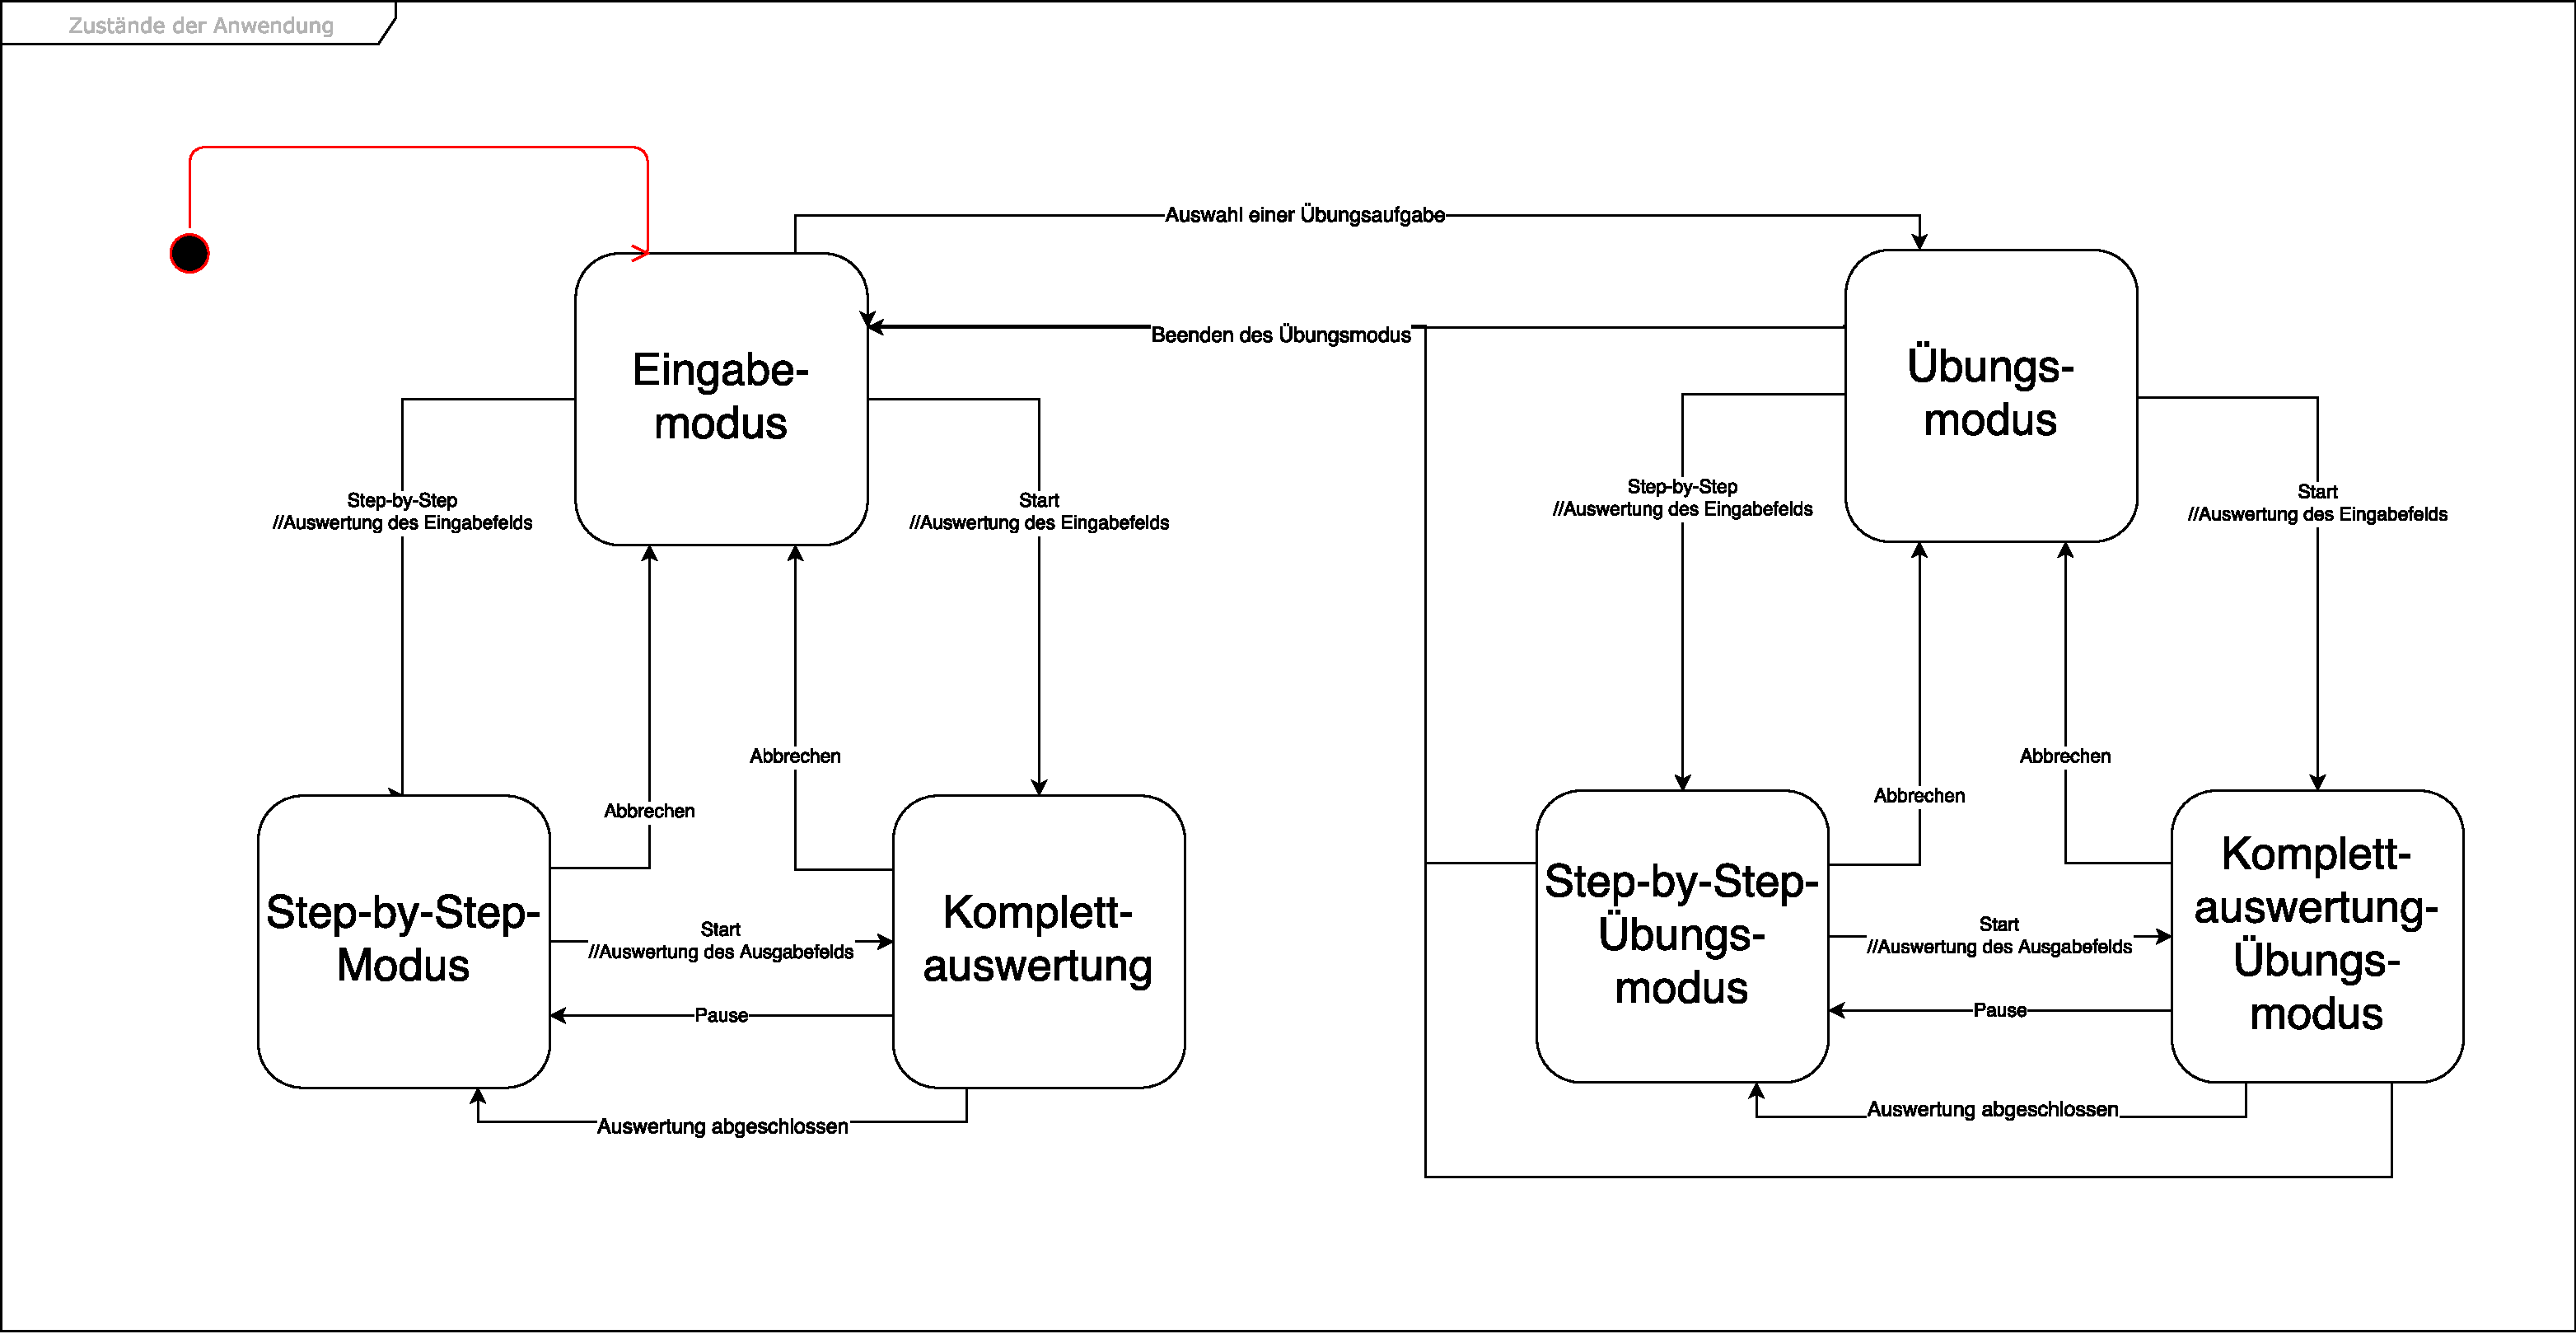
\includegraphics[width=\textwidth]{img/Zustandsautomat}
	\caption{\label{fig:state} Zustandsautomat der Anwendung}
\end{figure}

%Alternative zu hyperref?
Die Anwendung kann sich in drei verschiedenen Zuständen befinden, wobei jeder Zustand ein Gegenstück im \hyperref[fnc:ex]{Übungsmodus} besitzt. 
Der Übungsmodus wird durch Auswahl einer Übungsaufgabe betreten und durch Beendigung des Übungsmodus verlassen.\\
Beim Start der Anwendung befindet sich der Nutzer im Eingabemodus. In diesem Modus kann der Nutzer einen \gls{lt} in das Eingabefeld eingeben. 
Durch Drücken des Schritt-für-Schritt- oder Start-Knopfes (\cref{fig:actionButtons}) gelangt der Nutzer in den jeweiligen Auswertungsmodus und es beginnt die Auswertung des eingegebenen \glslink{lt}{$\lambda$-Terms}. 
Zeitgleich wird das Eingabefeld deaktiviert. Wenn noch Ausgaben einer früheren Auswertung im Ausgabefeld stehen, werden diese gelöscht.\\ 
Durch Drücken des Start- oder Pause-Knopfes kann der Nutzer zwischen den entsprechenden Auswertungsmodi wechseln. 
Beim Wechsel vom Schritt-für-Schritt-Modus zur Komplettauswertung wird der zuletzt ausgegebene \gls{lt} des Ausgabefeldes weiter ausgewertet.
Die Auswertungsmodi können erst durch das Drücken des Abbrechen-Knopfes verlassen werden. Es erscheint eine entsprechende Ausgabe im Ausgabefeld. Erst jetzt kann der Nutzer neue Eingaben im Eingabefeld eingeben.


%%%%%%%%%%%
\section{Tests}

\test{Komplettauswertung}{tst:complete}
\tests{fnc:ed}
\tests{fnc:completereduce}
\tests{fnc:live}

\teststep{Nutzer "Stephen Cook" hat einen Browser geöffnet.}
{Stephen navigiert zur URL des Wavelength-Projekts.}
{Die IDE öffnet sich wie in Abbildung~\ref{img:start}.}

\teststep{Die IDE ist fertig geladen.}
{Stephen gibt im Eingabefeld einen gültigen \gls{lt} mit Klammern ein,
dessen Reduktion durch die \gls{nr} terminiert.
Hierbei navigiert er über den Text und macht eine vermeintlich fehlerbehaftete Änderung rückgängig. 
Stephen merkt, dass die Änderung doch korrekt war und springt wieder zum aktuellen Stand. Er kopiert etwas Text und fügt diesen an einer anderen Stelle wieder ein.
Der \gls{lt} ist mehrere Zeilen lang und Stephen rückt mehrere Zeilen des \gls{lt}s gleichzeitig ein.
Stephen fügt eine neue Zeile hinter einer bereits eingerückten Zeile ein.}
{Das Textfeld verhält sich wie erwartet.}

\teststep{Als Ausgabeformat ist die Unicode-Ausgabe, als \gls{aws} die \gls{nr} und
als Ausgabeumfang die Ausgabe aller Teilschritte vorausgewählt.}
{Stephen betätigt den "Start"-Knopf.}
{Das Ausgabefeld füllt sich graduell mit den Zwischenschritten, welche gemäß der \glslink{nr}{normalen Reduktionsordnung} auftreten.
Zum Schluss wird die Normalform des eingangs eingegebenen Terms ausgegeben.}

\test{Schritt-für-Schritt-Modus}{tst:steps}
\tests{fnc:awsstrats}
\tests{fnc:steps}
% fehlt: \tests{fnc:interactive}

\teststep{Benutzer "Donald Knuth" befindet sich auf der Wavelength-Seite.}
{Er gibt einen syntaktisch korrekten \gls{lt} in das Eingabefeld ein und betätigt
den "Schritt-für-Schritt"-Knopf.}
{Der eingegebene Term wird in das Ausgabefeld übernommen und der Vor-Knopf wird aktiv. Im Term wird der nächste $\beta$-Reduktionsschritt
gemäß der \glslink{nr}{normalen Reduktionsordnung} markiert.}

\teststep{Die IDE befindet sich im Schritt-für-Schritt-Modus.}
{Don betätigt den "Vor"-Knopf.}
{Das Resultat der markierten Reduktion erscheint als neue Zeile im Ausgabefeld.
In der neuen Zeile ist der nächste Reduktionsschritt markiert.}

\teststep{Die IDE ist bereit für die nächste Eingabe.}
{Don betätigt den "Zurück"-Knopf.}
{Der zweite Reduktionsschritt wird aus dem Ausgabefeld entfernt.}

\teststep{Die IDE ist bereit für die nächste Eingabe.}
{Don schwebt mit der Maus über einem nicht markierten, zu einem \gls{redex} gehörenden
$\lambda$-Symbol in der aktiven Zeile im Ausgabefeld.}
{Die alten Markierungen in der aktiven Zeile verschwinden. Neue Markierungen für den \gls{redex}, über dem
sich die Maus befindet, erscheinen.}

\teststep{Der Mauszeiger befindet sich über einem Redex.}
{Don bewegt die Maus von diesem Redex weg.}
{Die Markierungen verschwinden und die Markierungen gemäß der \glslink{nr}{normalen Reduktionsordnung}
werden wieder angezeigt.}

\teststep{Die IDE ist bereit für die nächste Eingabe.}
{Don klickt mit der Maus auf ein zu einem \gls{redex} gehörendes $\lambda$-Symbol.}
{Es erscheint eine neue Zeile im Ausgabefeld, die das Ergebnis der angeklickten
Reduktion enthält. In der neuen Zeile erscheinen die Markierungen gemäß der ausgewählten
\gls{aws}.}

\teststep{Die IDE ist bereit für die nächste Eingabe.}
{Don wählt das Dropdown-Menü für die \gls{aws} an. Er wählt "\gls{cbn}".}
{Die Markierungen für die vorher ausgewählte \gls{aws} werden ausgeblendet.
Stattdessen wird der nächste Schritt gemäß \gls{cbn} angezeigt.}

\teststep{Die IDE ist bereit für die nächste Eingabe.}
{Don betätigt den "Vor"-Knopf.}
{Das Resultat der markierten Reduktion (gemäß \gls{cbn}) erscheint als neue Zeile im Ausgabefeld.
In der neuen Zeile wird der nächste Reduktionsschritt markiert.}

\teststep{Die IDE ist bereit für die nächste Eingabe.}
{Don wiederholt die vorangegangenen beiden Schritte für "\gls{cbv}" und "\gls{ao}".}
{Die Applikation verhält sich wie in den vorherigen beiden Schritten beschrieben,
verwendet aber die jeweils ausgewählte \gls{aws}.}

\test{Erstellen vom Permalinks}{tst:perma}
\tests{fnc:perma}
\tests{fnc:steps}

\teststep{Benutzer "Edsger Dijkstra" befindet sich auf der Wavelength-Seite.}
{Edsger gibt einen gültigen \gls{lt} in die Software ein, wählt eine \gls{aws} und ein
Ausgabeformat aus, begibt sich in den Schritt-für-Schritt-Modus und durchläuft einige
Schritte der Auswertung.}
{Die Anwendung verhält sich wie spezifiziert.}

\teststep{Die IDE ist bereit für die nächste Aktion.}
{Edsger verwendet den "Teilen"-Knopf im unteren Bereich der Anwendung.}
{Neben dem Knopf erscheint eine URL wie in Abbildung~\ref{img:share}
abgebildet.}

\teststep{Edsger hat die URL in seine Zwischenablage kopiert.}
{Edsger wählt die URL in einem neuen Browserfenster an.}
{Die IDE öffnet sich im neuen Fenster und Eingabefeld, Ausgabefeld und alle Optionen befinden sich im gleichen Zustand wie im alten Fenster.}

\teststep{Die IDE ist im neuen Fenster geöffnet.}
{Edsger betätigt den "Zurück"-Knopf.}
{Der letzte im alten Browserfenster durchgeführte Schritt wird im neuen Browserfenster
rückgängig gemacht.}

\test{Übungsmodus}{tst:ex}
\tests{fnc:ex}

\teststep{Benutzerin "Ada Lovelace" befindet sich auf der Wavelength-Seite.}
{Ada wählt im Menü (vgl. \cref{fig:exerciseMode}) eine Übungsaufgabe aus.}
{Es öffnet sich ein Fenster, das Ada darauf hinweist, dass ihre Eingabe und Ausgabe verloren geht.
 Ada wählt "fortfahren" aus.
 Der Übungsmodus wird aktiviert. 
 Das Eingabefeld wird aufgeteilt in ein schmaleres Eingabefeld und ein Aufgabenfeld.
 Im Aufgabenfeld erscheint eine Beschreibung der gewählten \gls{ex}.
 Der "Beenden"- und der "zeige Lösung"-Knopf erscheinen.}

\teststep{Die IDE ist bereit für die nächste Aktion.}
{Ada gibt eine syntaktisch korrekte Lösung ein, die kein korrektes Ergebnis liefert.
 Ada drückt den "Start"-Knopf.}
{Die IDE wertet die Eingabe wie spezifiziert aus.
 Nach dem letzten Schritt wird angezeigt, dass die Lösung inkorrekt ist.}

\teststep{Die IDE ist bereit für die nächste Aktion.}
{Ada gibt die korrekte Lösung ein. Ada drückt den "Start"-Knopf.}
{Die IDE wertet die Eingabe wie spezifiziert aus.
 Nach dem letzten Schritt wird angezeigt, dass die Lösung korrekt ist.}
 
\teststep{Die IDE ist bereit für die nächste Aktion.}
{Ada wählt eine andere Übungsaufgabe aus und bestätigt, dass Eingabe- und Ausgabe verloren gehen.}
{Eingabe und Ausgabe werden entfernt.
Im Aufgabenfeld erscheinen eine Beschreibung der \gls{ex} und ein Stück Code.}

\teststep{Die IDE ist bereit für die nächste Aktion.}
{Ada vervollständigt den Code zu einer korrekten Lösung und durchläuft den Schritt-für-Schritt-Modus komplett von Hand.}
{Die IDE verhält sich wie spezifiziert.
 Als letzter Schritt wird angezeigt, dass die eingegebene Lösung korrekt ist.}

\teststep{Die IDE ist bereit für die nächste Aktion.}
{Ada drückt auf den "zeige Lösung"-Knopf.}
{Die Musterlösung wird im Aufgabenfeld angefügt.
 Der "zeige Lösung"-Knopf wird zum "verberge Lösung"-Knopf.}

\teststep{Im Aufgabenfeld wird die Musterlösung angezeigt.}
{Ada kopiert die Musterlösung, überschreibt ihre Eingabe damit und drückt den "Start"-Knopf.}
{Die IDE verhält sich wie spezifiziert. 
 Als letzter Schritt wird angezeigt, dass die eingegebene Lösung korrekt ist.}
 
\teststep{Die IDE ist bereit für die nächste Aktion.}
{Ada drückt auf den "verberge Lösung"-Knopf.}
{Die Musterlösung wird aus dem Aufgabenfeld entfernt.}
 
\teststep{Die IDE ist bereit für die nächste Aktion.}
{Ada drückt den "Beenden"-Knopf.}
{Es öffnet sich ein Fenster, das Ada darauf hinweist, dass ihre Eingabe und Ausgabe verloren geht.
 Ada wählt "fortfahren" aus.
 Der Übungsmodus wird beendet, der "Beenden"-Knopf verschwindet, Eingabe und Ausgabe werden entfernt.
 Das Aufgabenfeld wird entfernt.}

\test{Ausgabeformate}{tst:display}
\tests{fnc:display}
\tests{fnc:unicode}
\tests{fnc:tree}

\teststep{Benutzer "Richard Hamming" befindet sich auf der Wavelength-Seite.}
{Richard gibt einen syntaktisch korrekten \gls{lt} ein und drückt den "Start"-Knopf.}
{Der eingegebene \gls{lt} wird ausgewertet und im Unicode-Format im Ausgabefeld angezeigt.}

\teststep{Im Ausgabefeld wird das Ergebnis der vorherigen Schritts angezeigt.}
{Richard bewegt den Mauszeiger auf eine öffnende Klammer in der letzten Zeile der Ausgabe.}
{Die öffnende Klammer und die zugehörige schließende Klammer werden markiert.}

\teststep{Die IDE ist bereit für die nächste Aktion}
{Richard wählt im Dropdown-Menü (vgl. \cref{fig:display}) das Ausgabeformat "tree" und drückt den "Start"-Knopf.}
{Der eingegebene \gls{lt} wird ausgewertet und wie spezifiziert(vgl. \ref{fnc:tree}) ausgegeben.}

\test{Export}{tst:output}
\tests{fnc:output}

\teststep{Benutzer "Robert Tarjan" befindet sich auf der Wavelength-Seite.}
{Robert gibt einen gültigen \gls{lt} ein und drückt auf den "Exportieren"-Knopf.}
{Es öffnet sich eine Liste mit allen Exportformaten.}

\teststep{Die IDE erwartet die Auswahl eines Exportformats.}
{Robert wählt ein beliebiges Exportformat aus der Liste aus.}
{Die Liste mit den Exportformaten verschwindet.
Es öffnet sich ein Fenster (vgl. \cref{fig:export}) mit der formatierten Eingabe.}

\teststep{Robert ist im Fenster mit der formatierten Eingabe.}
{Robert kopiert die formatierte Eingabe und schließt das Fenster.}
{Das Fenster mit der formatierten Eingabe verschwindet. 
 Die Eingabe aus dem ersten Schritt ist noch im Eingabefeld.}
 
\test{Namensbindung}{tst:bind}
\tests{fnc:bind}
\tests{fnc:diag}

\teststep{Benutzer "Haskell Curry" befindet sich auf der Wavelength-Seite.}
{Haskell gibt einen gültigen \gls{lt} ein und nennt ihn "curry".
 Haskell verwendet "curry" in einem weiteren gültigen \gls{lt} und drückt den "Start"-Knopf.}
{Die Eingabe wird gemäß Spezifikation ausgewertet (vgl. \gls{nb}).}

\teststep{Die IDE ist bereit für die nächste Aktion.}
{Haskell gibt einen gültigen \gls{lt} ein.
 Er benennt ihn mit einem gemäß Spezifikation (vgl. \gls{nb}) ungültigen Namen.
 Er drückt den "Start"-Knopf.}
{Es wird eine Fehlermeldung ausgegeben.
 Haskell wird darauf hingewiesen, dass er einen ungültigen Namen gewählt hat.}

\teststep{Die IDE ist bereit für die nächste Aktion.}
{Haskell bindet zwei gültige \glspl{lt} an den gleichen Namen und drückt den "Start"-Knopf.}
{Es wird eine Fehlermeldung ausgegeben. Haskell wird darauf hingewiesen, dass Namen
nur einmal gebunden werden dürfen.}

\test{Auswahl des Ausgabeumfangs}{tst:selectsize}
\tests{fnc:selectsize}

\teststep{Benutzer "Wilhelm Ackermann" befindet sich auf der Wavelength-Seite.}
{Wilhelm gibt einen gültigen \gls{lt} ein und drückt auf den "Start"-Knopf. }
{Die Eingabe wird ausgewertet und nur das Ergebnis wird angezeigt (vgl. \gls{std}).}

\teststep{Die IDE ist bereit für die nächste Aktion.}
{Wilhelm wählt im Ausgabeumfang-Dropdown-Menü einen anderen Ausgabeumfang aus (vgl. \ref{fig:outputOptions}) und drückt auf den "Start"-Knopf.}
{Die IDE verhält sich wie spezifiziert (vgl. \ref{fnc:selectsize}).}

\teststep{Die IDE ist bereit für die nächste Aktion.}
{Wilhelm wählt in der "Display"-Box das Ausgabeformat "Tree" und drückt den "Start"-Knopf.}
{Die IDE verhält sich wie spezifiziert (vgl. \ref{fnc:completereduce}).
 Im Ausgabefeld erscheint ein Syntaxbaum gemäß des ausgewählten Ausgabeumfangs (vgl. \ref{fnc:tree}).}
 
\test{Wechsel des Auswertungsmodus}{test:changemodes}
\tests{fnc:cancel}

\teststep{Die \gls{cmpltapp} eines korrekten \glslink{lt}{$\lambda$-Terms} läuft.}
{Nutzer "Bob" drückt den "Pause"-Knopf.}
{Die Auswertung wird angehalten, der aktuelle \gls{lt} wird in das Ausgabefeld geschrieben, die IDE wechselt in den Schritt-für-Schritt-Modus.}

\teststep{Die IDE befindet sich im Schritt-für-Schritt-Modus.}
{Bob drückt den "Start"-Knopf.}
{Die IDE wechselt in den Komplettauswertungs-Modus, der eingegebene \gls{lt} wird ohne Aktionen des Nutzers ausgewertet.}

\teststep{Die \gls{cmpltapp} eines \glslink{lt}{$\lambda$-Terms} läuft.}
{Bob drückt den "Abbrechen"-Knopf.}
{Die Auswertung wird abgebrochen, das Ausgabefeld wird erhalten und deaktiviert, das Eingabefeld kann bearbeitet werden.}
 
\test{Standardbibliothek}{test:lib}
\tests{fnc:lit}
\tests{fnc:lib}

\teststep{Benutzer "Alan Turing" befindet sich auf der Wavelength-Seite.}
{Alan wählt im Menü die \gls{yc}-Bibliothek aus.}
{Die gewählte Bibliothek wird geladen.}

\teststep{Die Basisbibliothek ist eingebunden.}
{Alan benutzt den \gls{yc} in einem gültigen \gls{lt} und drückt den "Start"-Knopf.}
{Die IDE verhält sich wie spezifiziert.}

\teststep{Die natürlichen Zahlen sind eingebunden.}
{Alan definiert eine natürliche Zahl durch ein \gls{lit}.
 Für diese Zahl benutzt er die Funktionen, um Vorgänger und Nachfolger zu bestimmen.
 Dann drückt er den "Start"-Knopf.}
{Die IDE verhält sich wie spezifiziert.}

\teststep{Die natürlichen Zahlen sind eingebunden.}
{Alan verrechnet zwei natürliche Zahlen mit den gegebenen Operationen (siehe \ref{fnc:lib}).}
{Die IDE verhält sich wie spezifiziert.}

\teststep{Die natürlichen Zahlen sind eingebunden.}
{Alan gibt den Term \emph{"($\lambda$x.2x) (3)"} ein und drückt den "Start"-Knopf.}
{Es wird \emph{"6"} ausgegeben.}

\teststep{Die Wahrheitswerte sind eingebunden.}
{Alan definiert zwei gültige \glspl{lt} a und b.
 Alan gibt ein: "true a b" und drückt den "Start"-Knopf.}
{Es wird "a" ausgegeben.}

\teststep{Die Wahrheitswerte sind eingebunden.}
{Alan definiert zwei gültige \glspl{lt} a und b.
 Alan gibt ein: "false a b" und drückt den "Start"-Knopf.}
{Es wird "b" ausgegeben.}

\teststep{Tupel und Listen sind eingebunden.}
{Alan erschafft ein Tupel und benutzt die Funktionen car bzw. cdr (siehe \ref{fnc:lib}).
 Er drückt den "Start"-Knopf.}
{Es wird das erste bzw. das zweite Element des Tupels ausgegeben.}

\teststep{Tupel und Listen sind eingebunden.}
{Alan erschafft eine leere Liste \emph{list} mit \emph{null}. 
 Mit dem Befehl \emph{cons a list} hängt er das Element \emph{a} an den Anfang von \emph{list} und bindet das Resultat
 an den Namen \emph{list2}.
 Mit dem Befehl \emph{cons b list2} hängt er das Element \emph{b} an den Anfang von \emph{list2} und bindet das
 Resultat an den Namen \emph{list3}.
 Alan benutzt die Funktionen \emph{car} und \emph{cdr} (siehe \ref{fnc:lib}), um das erste bzw. zweite Element von \emph{list3}
 zu erhalten
 und drückt den "Start"-Knopf.}
{Es wird \emph{a} bzw. \emph{b} ausgegeben.}

\test{Fehlerdiagnostik}{tst:diag}
\tests{fnc:diag}

\teststep{Benutzer "Richard Bellman" befindet sich auf der Wavelength-Seite.}
{Richard gibt einen syntaktisch inkorrekten \gls{lt} ein, der eine schließende Klammer
zu wenig enthält und wählt den "Start"-Knopf an.}
{Im Ausgabefeld wird eine Nachricht angezeigt, die auf unbalancierte Klammerung hinweist.
Die Nachricht enthält einen Vorschlag für einen korrigierten Term. Im Eingabefenster wird
die Klammer, die keinen Partner besitzt, markiert.}

\teststep{Die IDE ist bereit für die nächste Aktion.}
{Richard löscht die aktuelle Eingabe aus dem Eingabefenster und gibt einen inkorrekten Term ein, der strukturell weder \gls{lapp}, noch
\gls{labs}, noch \gls{var} ist. Dann wählt er den "Start"-Knopf an.}
{Im Ausgabefeld erscheint eine Nachricht, die darauf hinweist, dass der eingegebene
Term strukturell inkorrekt ist.}

\teststep{Die IDE ist bereit für die nächste Aktion.}
{Richard leert das Eingabefeld und wählt den "Start"-Knopf an.}
{Im Ausgabefeld erscheint eine Nachricht, die darauf hinweist, dass die Eingabe leer war.}

\teststep{Die IDE ist bereit für die nächste Aktion.}
{Richard gibt \emph{"//($\lambda$x.x) (5)"} in das Eingabefeld ein und drückt den "Start"-Knopf.}
{Im Ausgabefeld erscheint eine Nachricht, die darauf hinweist, dass die Eingabe leer war.}

\teststep{Die IDE ist bereit für die nächste Aktion.}
{Richard gibt zwei syntaktisch korrekte \glspl{lt}, die beide keine \gls{nb} sind, nacheinander
in das Eingabefeld ein und wählt den "Start"-Knopf an.}
{Im Ausgabefeld erscheint eine Nachricht, die darauf hinweist, dass eine gültige Eingabe
aus beliebig vielen Namensbindungen gefolgt von genau einem freistehendem \gls{lt} besteht.}
% Syntax:
% \test{Überschrift des Tests}{tst:label}
% \tests{fnc:label}
% \tests{nfc:label}
%
% \teststep{Stand}
% {Aktion}
% {Reaktion}
%
% \teststep{Stand}
% {Aktion}
% {Reaktion}
%
% ...

%%%%%%%%%%%%%
\pagebreak
\appendix

\section{Seitenentwürfe}


% Hier ganz normale figures mit Bildern
Bei Aufruf der Website wird eine leere IDE angezeigt. Das obere Textfeld ist das Eingabefeld, das untere ist das Ausgabefeld. Das Größenverhältnis der Felder kann mittels einer Schaltfläche angepasst werden.

\begin{figure}[H]
	\centering
	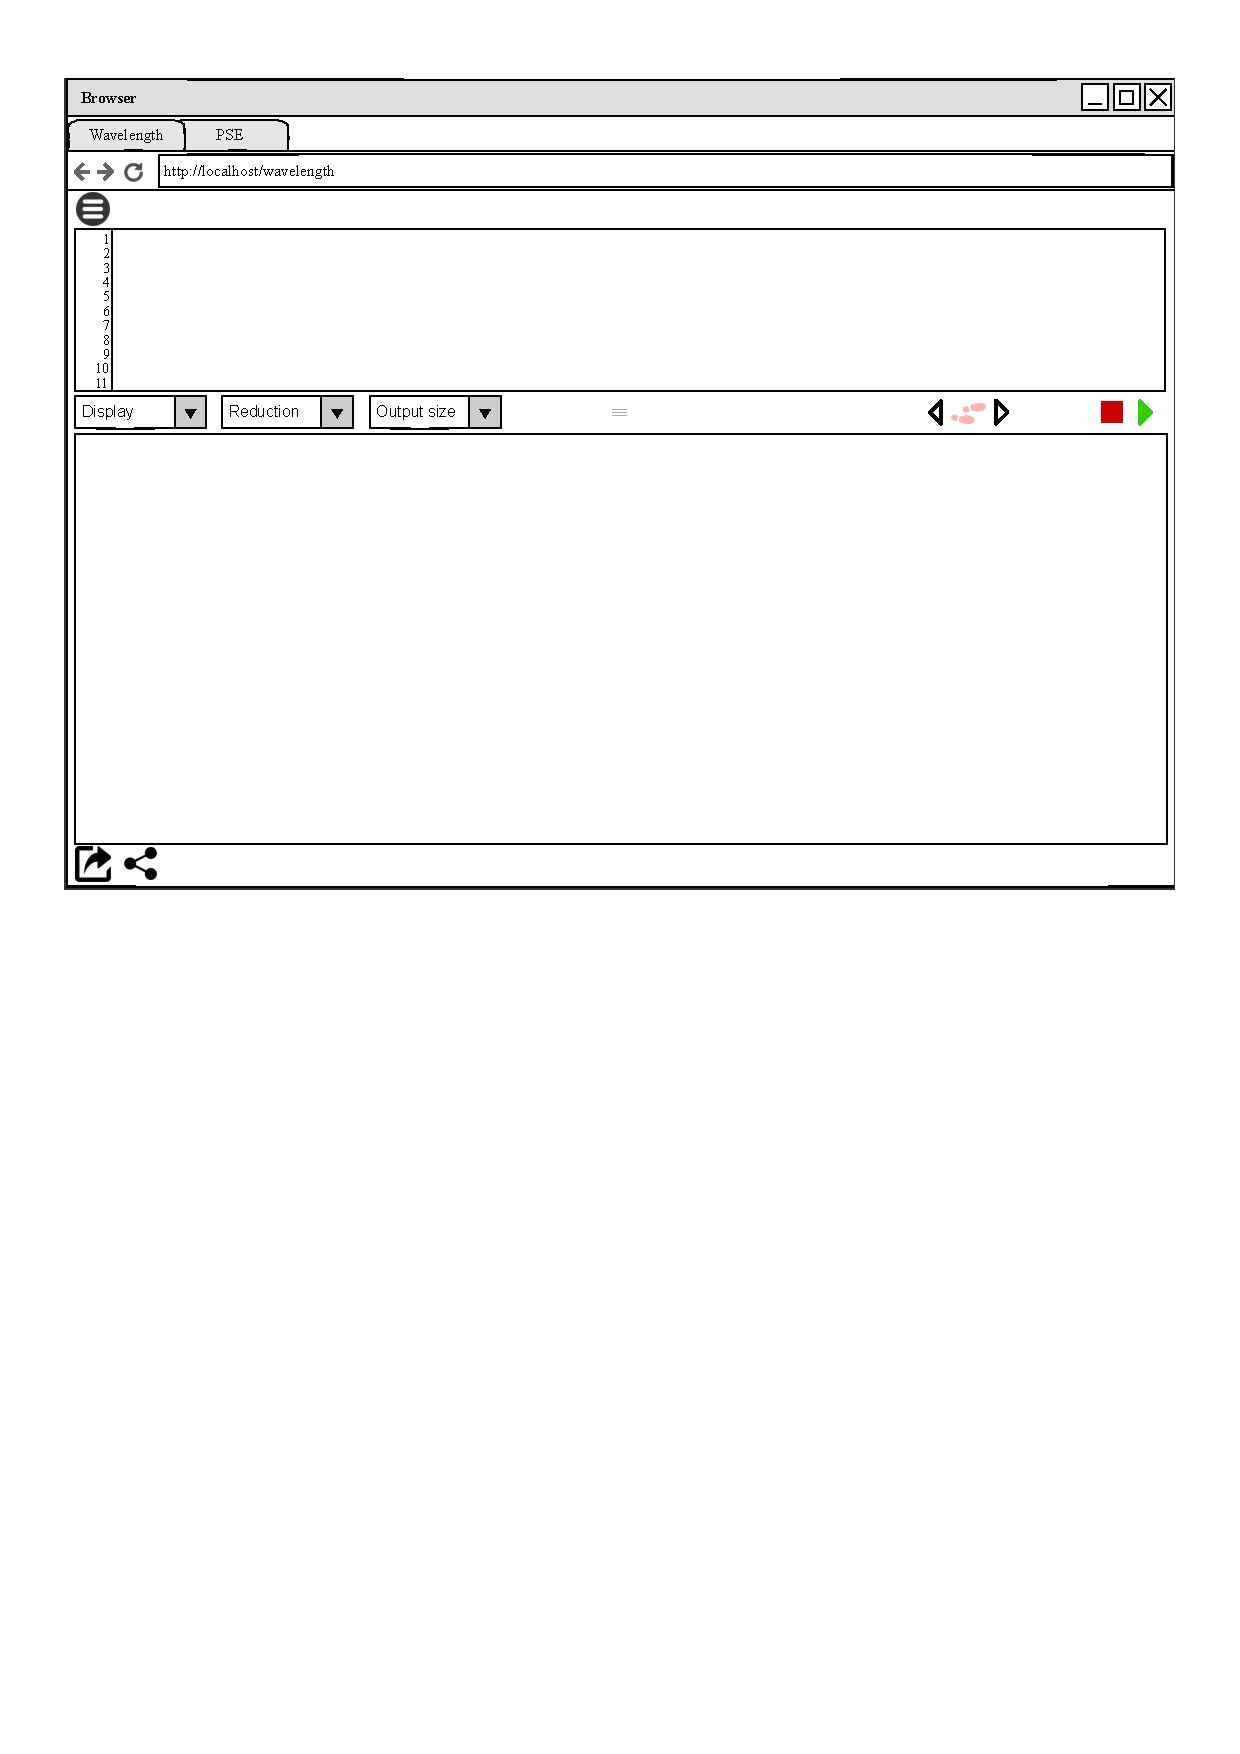
\includegraphics[width = \textwidth]{img/startseite}
	\caption{Die Startseite der IDE bei Aufruf der Website.} 
	\label{img:start}
\end{figure}


Der "Start"-Knopf löst die Auswertung zum Endergebnis aus. Durch Drücken des "Abbrechen"-Knopfes wird die Auswertung abgebrochen. Beim Drücken des Schritt-für-Schritt-Knopfes wird der Schritt-für-Schritt-Modus gestartet, in welchem der Nutzer mit den beiden Knöpfen daneben navigieren kann.

\begin{figure}[H]
	\centering
	
\includegraphics{img/actionButton}
	\caption{\label{fig:actionButtons} Schritt-zurück, Schritt-für-Schritt-Modus, 
	Schritt-vor, Start und Abbrechen (von links nach rechts)}
\end{figure}



\begin{figure}[H]
	\centering
	
\includegraphics{img/pauseButton}
	\caption{Wurde die Auswertung mittels "Start" gestartet, wird der "Start"-Knopf durch einen "Pause"-Knopf ersetzt, um in den Schritt-für-Schritt-Modus wechseln zu können.}
\end{figure}


\begin{figure}[H]
	\begin{subfigure}[l]{0.25\textwidth}
	\centering
		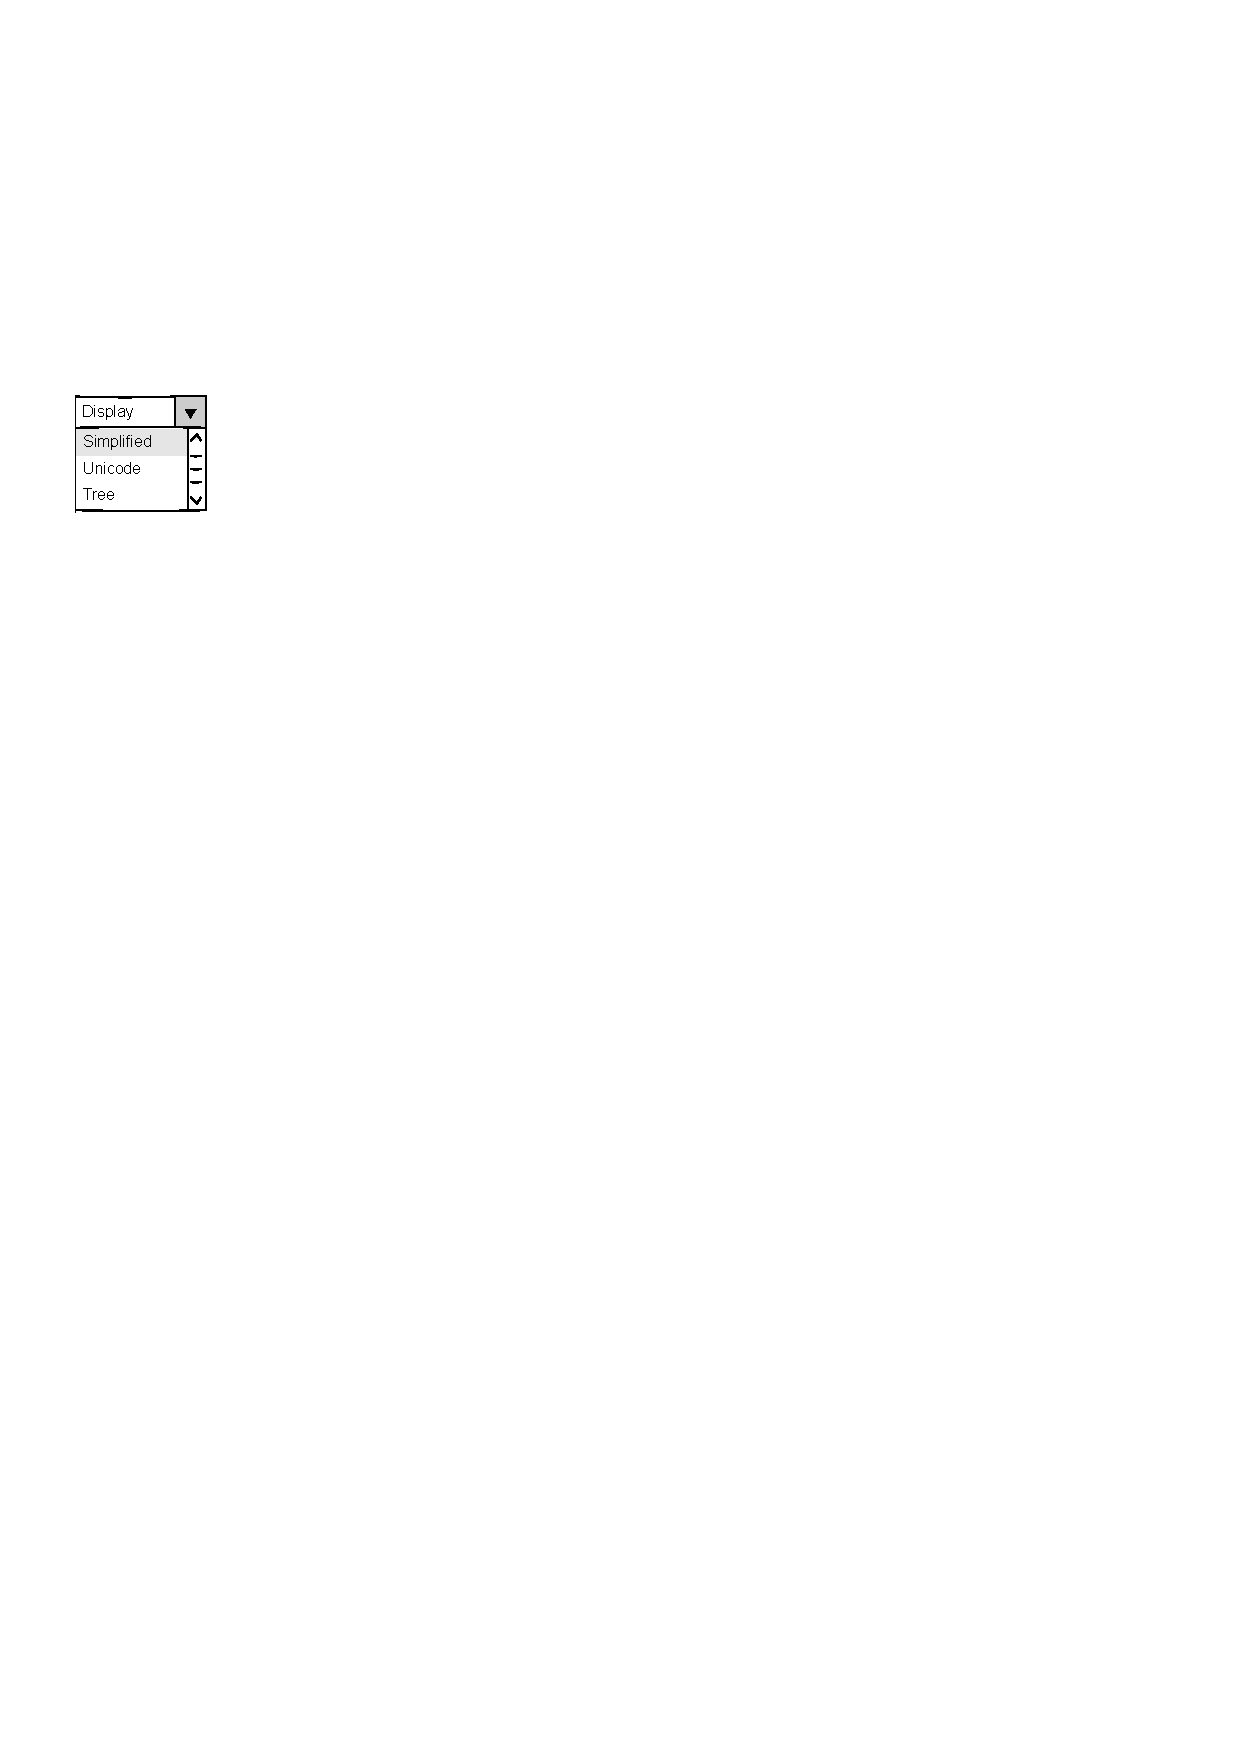
\includegraphics{img/displayMenu}
	\caption{\label{fig:display}Auswahl des Ausgabeformats}	
	\end{subfigure}
	\hspace*{\fill}
	\begin{subfigure}[m]{0.25\textwidth}
	\centering
		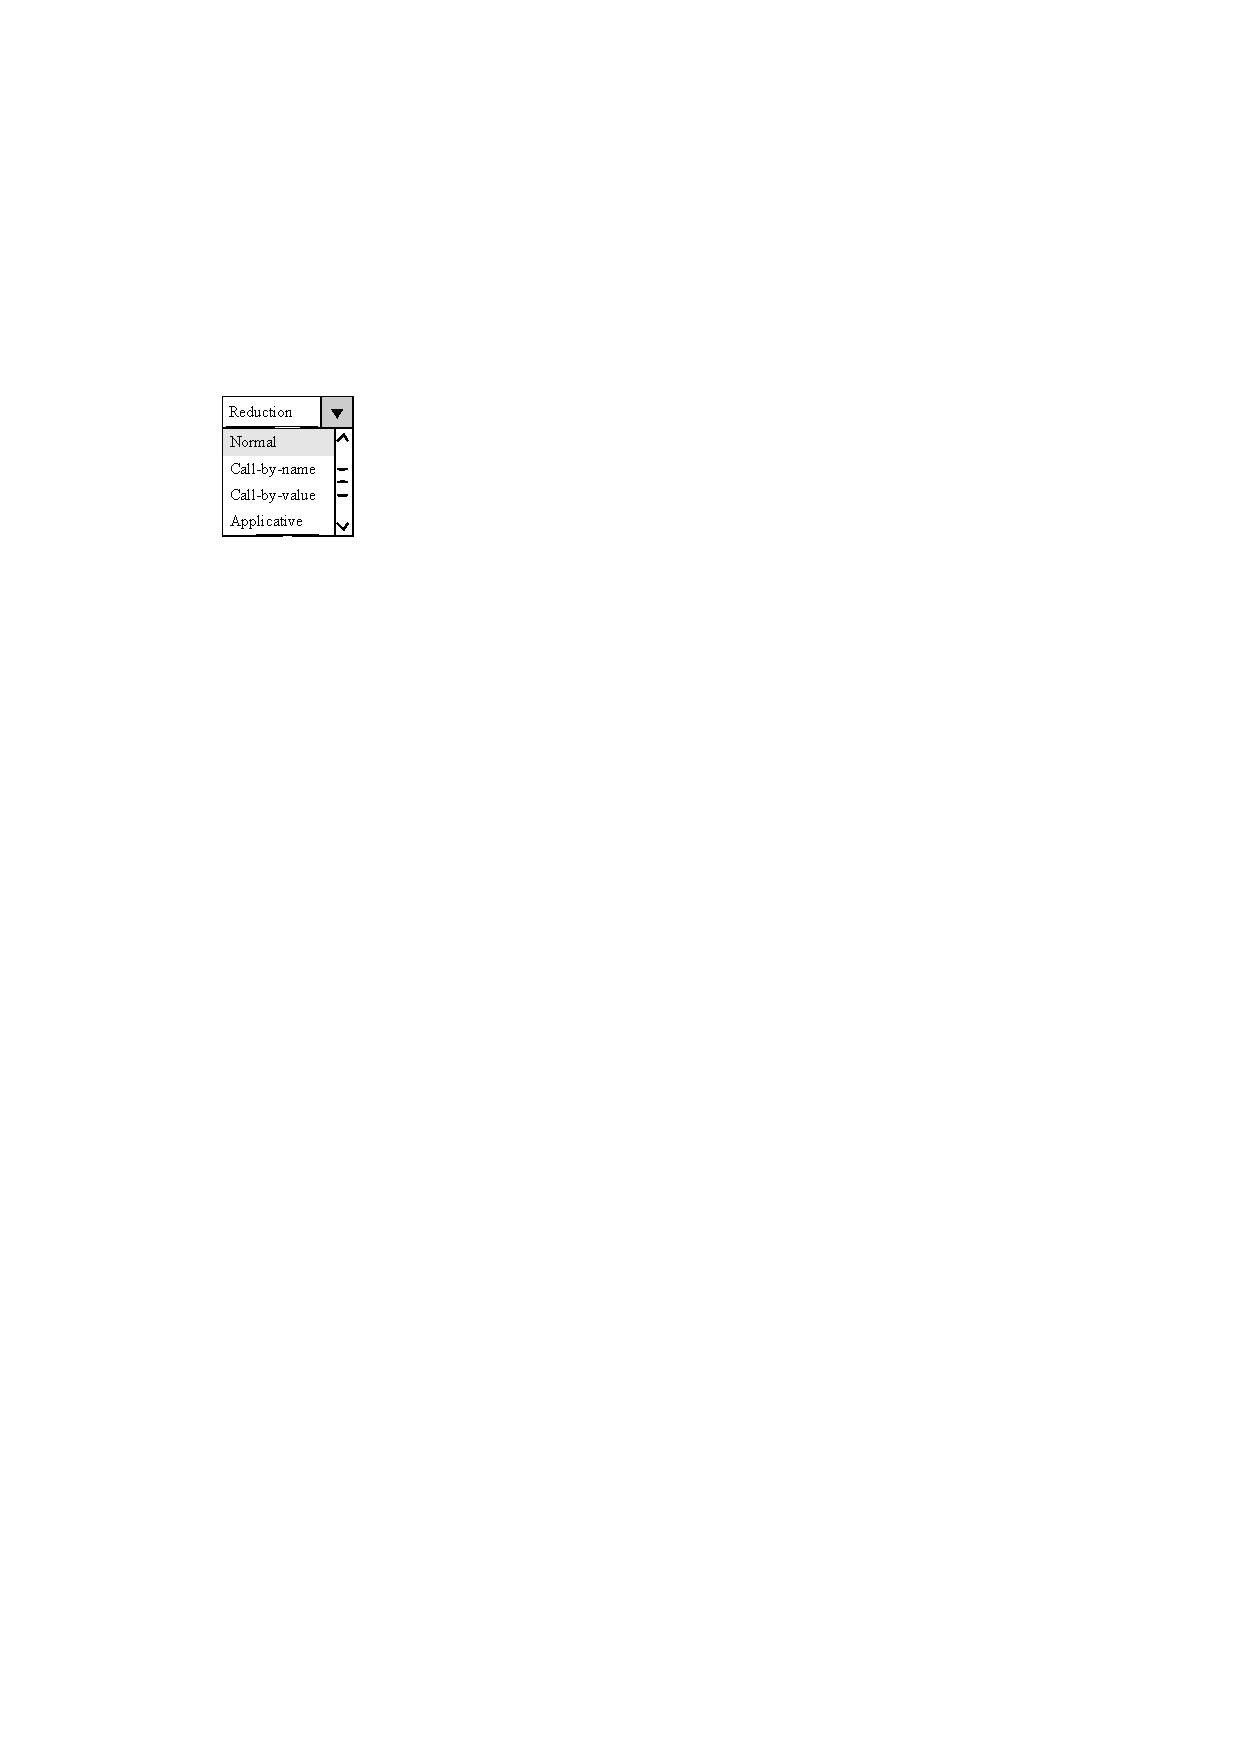
\includegraphics{img/reductionMenu}
	\caption{\label{fig:awsOptions}Auswahl der Auswertungsstrategie}
	\end{subfigure}
	\hspace*{\fill}
	\begin{subfigure}[r]{0.25\textwidth}
	\centering
		
\includegraphics{img/outputSizeMenu}
	\caption{Auswahl des Ausgabeumfangs}	
	\end{subfigure}
	\caption{\label{fig:outputOptions} Verschiedene Ausgabeoptionen können festgelegt werden.}
\end{figure}


\begin{figure}[H]
	\centering
	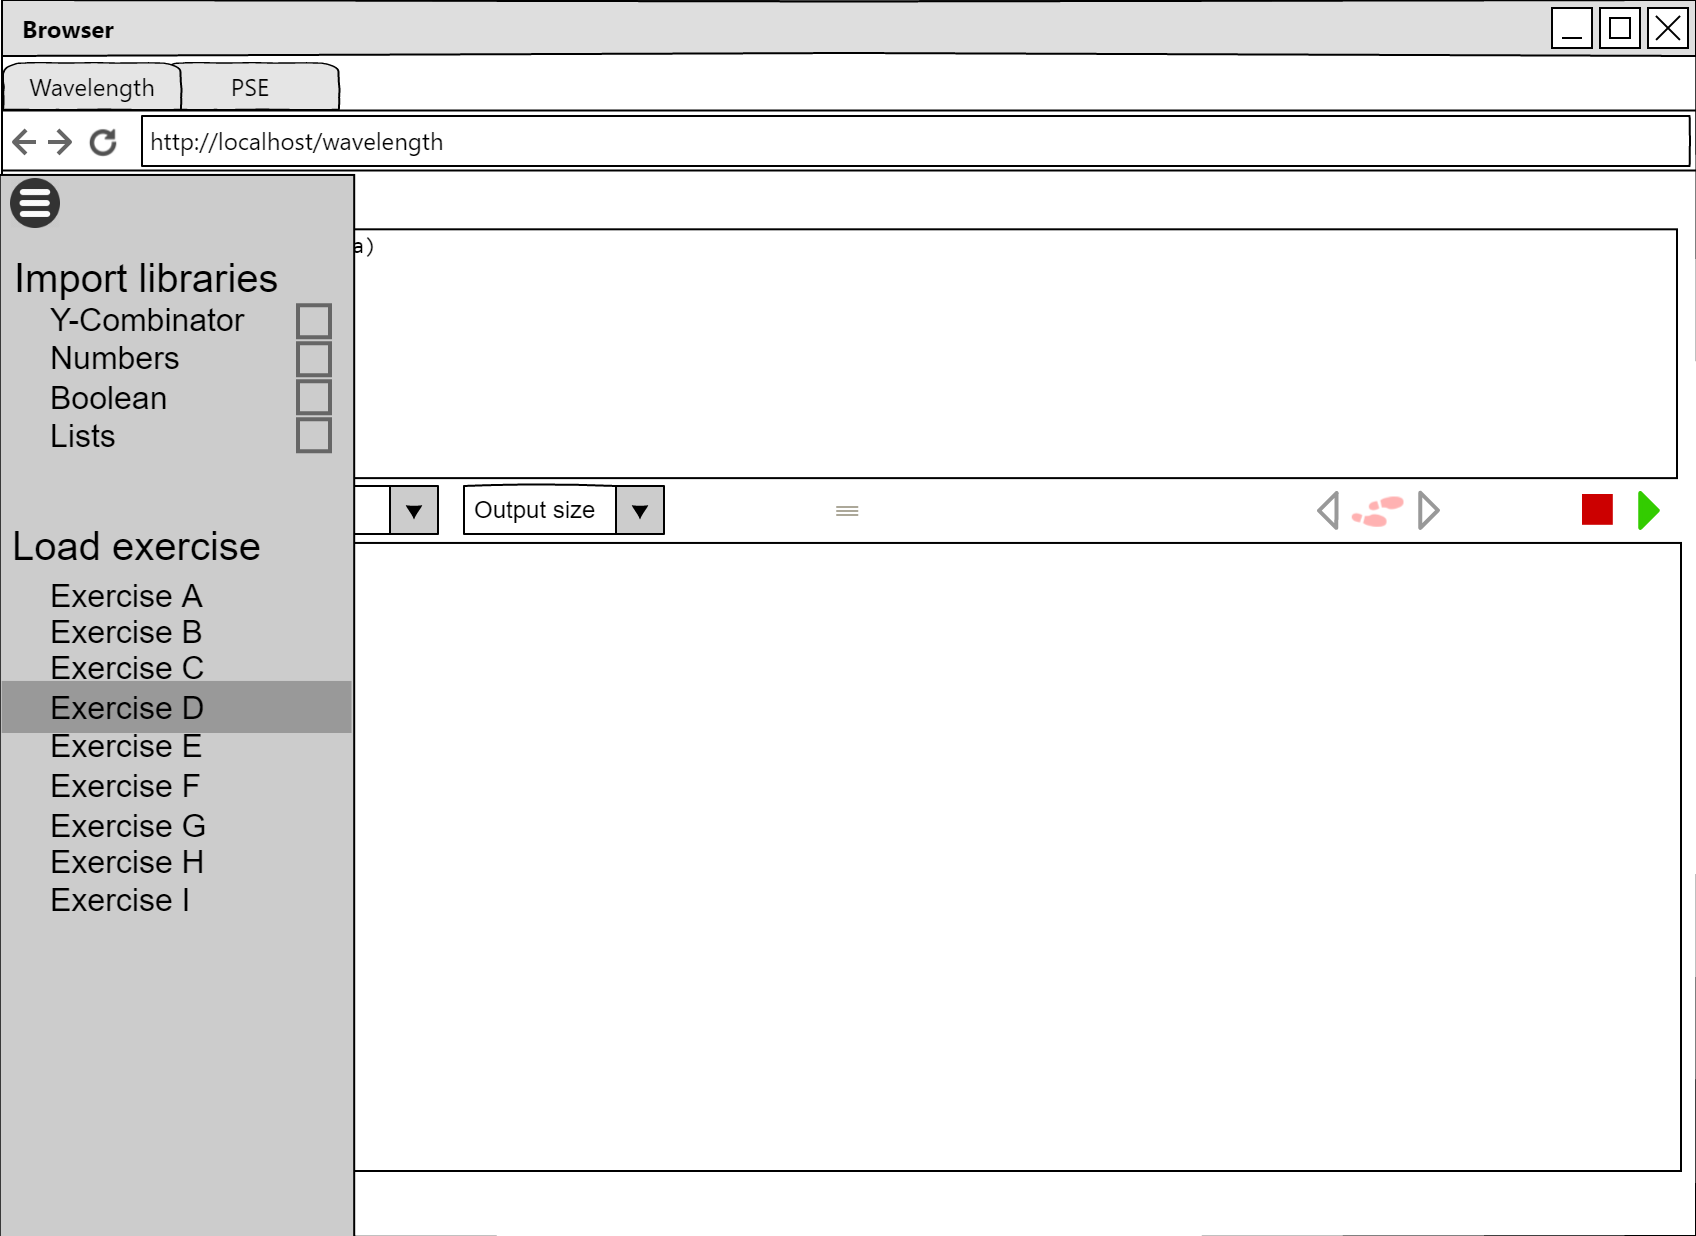
\includegraphics[width=\textwidth]{img/exercise_menue_open.png}
	\caption{\label{fig:exmenu}Im Optionsmenü hat der Nutzer die Möglichkeit, Bibliotheken einzubinden oder eine Übungsaufgabe auszuwählen.}
\end{figure}

\begin{figure}[H]
	\centering
	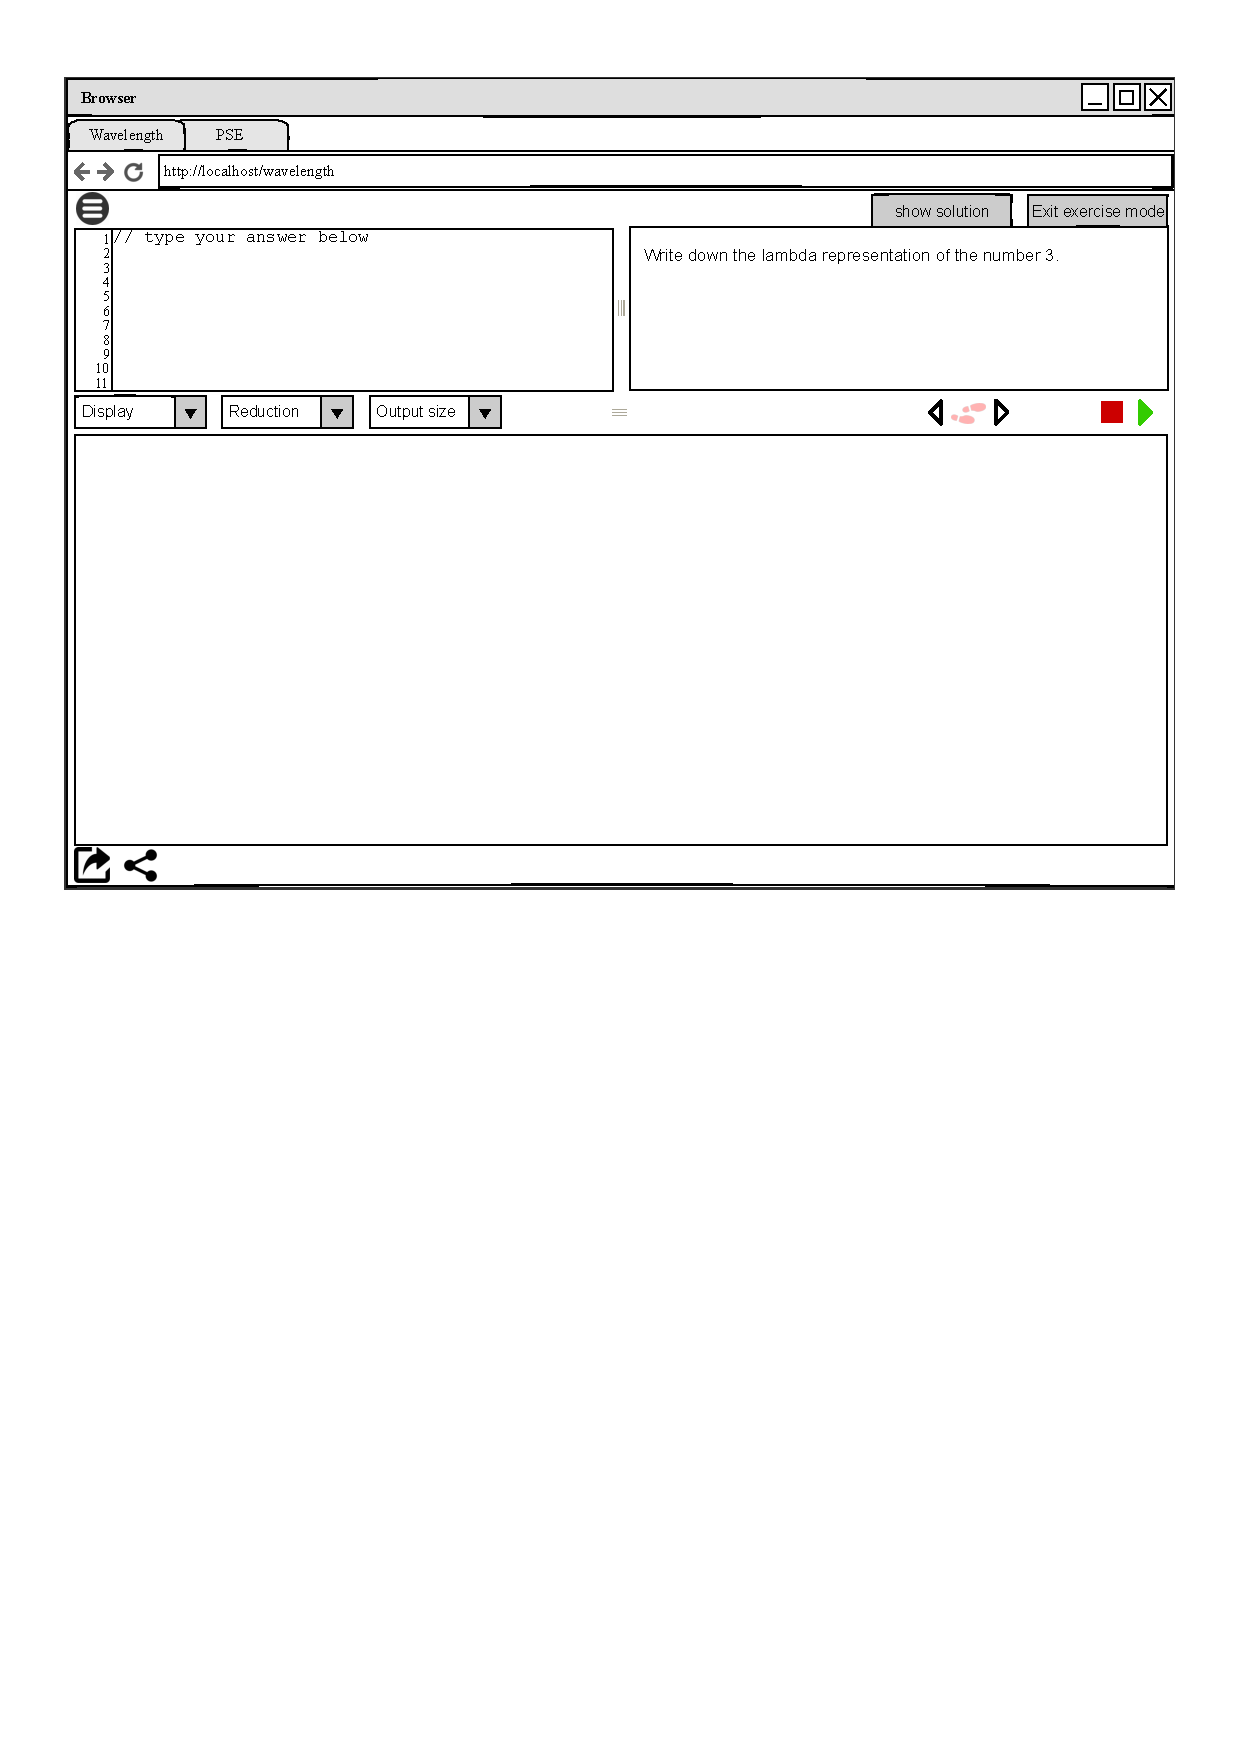
\includegraphics[width=\textwidth]{img/exerciseMode}
	\caption{\label{fig:exerciseMode}Wurde eine Übungsaufgabe ausgewählt, so wird die Aufgabenstellung im neu erscheinenden Aufgabenfeld angezeigt. Eventuell vorgegebene Eingaben werden in das Eingabefeld geladen. Der Nutzer hat die Möglichkeit, das Größenverhältnis dieser beiden Felder anzupassen. Die Musterlösung der Aufgabe wird durch Klicken eines entsprechenden Knopfes angezeigt oder auch wieder ausgeblendet. Mit Klick auf einen weiteren Knopf kann der Übungsmodus beendet werden.}
\end{figure}


\begin{figure}[H]
	\centering
	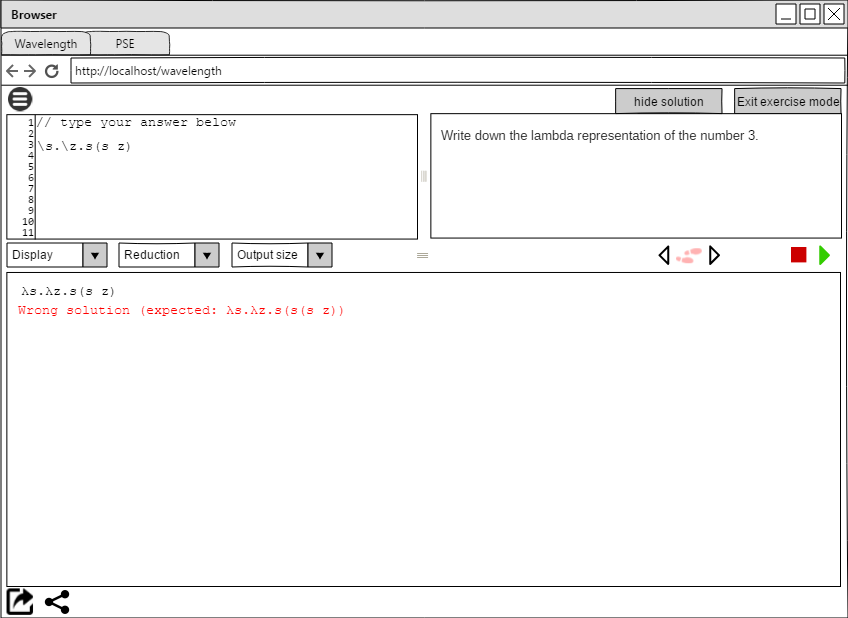
\includegraphics[width=\textwidth]{img/exercise_mode_solution_check.png}
	\caption{\label{fig:solutionCheck}Lässt der Nutzer seine Eingabe prüfen, so wird im Ausgabefeld angezeigt, ob diese korrekt ist.}
\end{figure}


\begin{figure}[H]
	\centering
	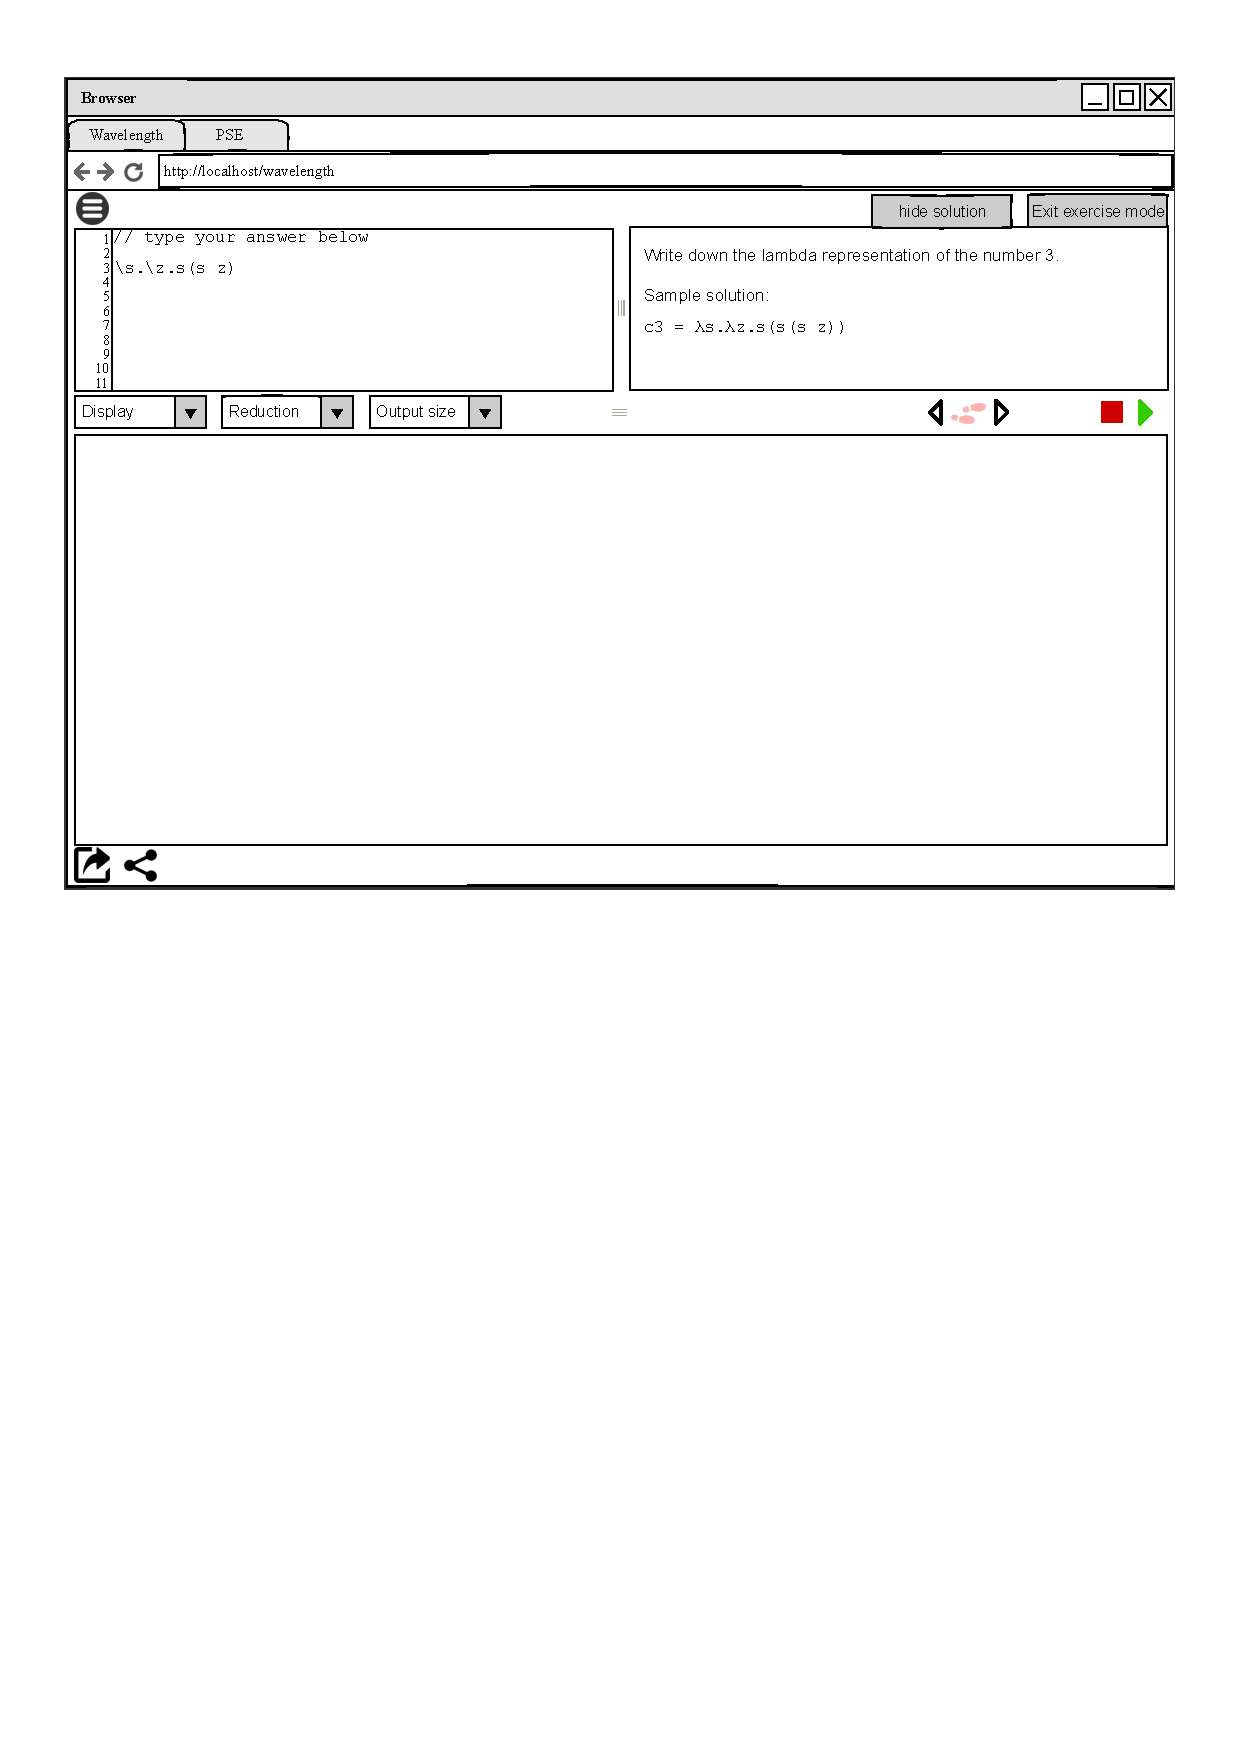
\includegraphics[width=\textwidth]{img/exerciseModeSolution}
	\caption{\label{fig:showSolution}Wird die Musterlösung angezeigt, so hat der Nutzer die Möglichkeit, diese auch wieder auszublenden.}
\end{figure}


\begin{figure}[H]
	\centering
	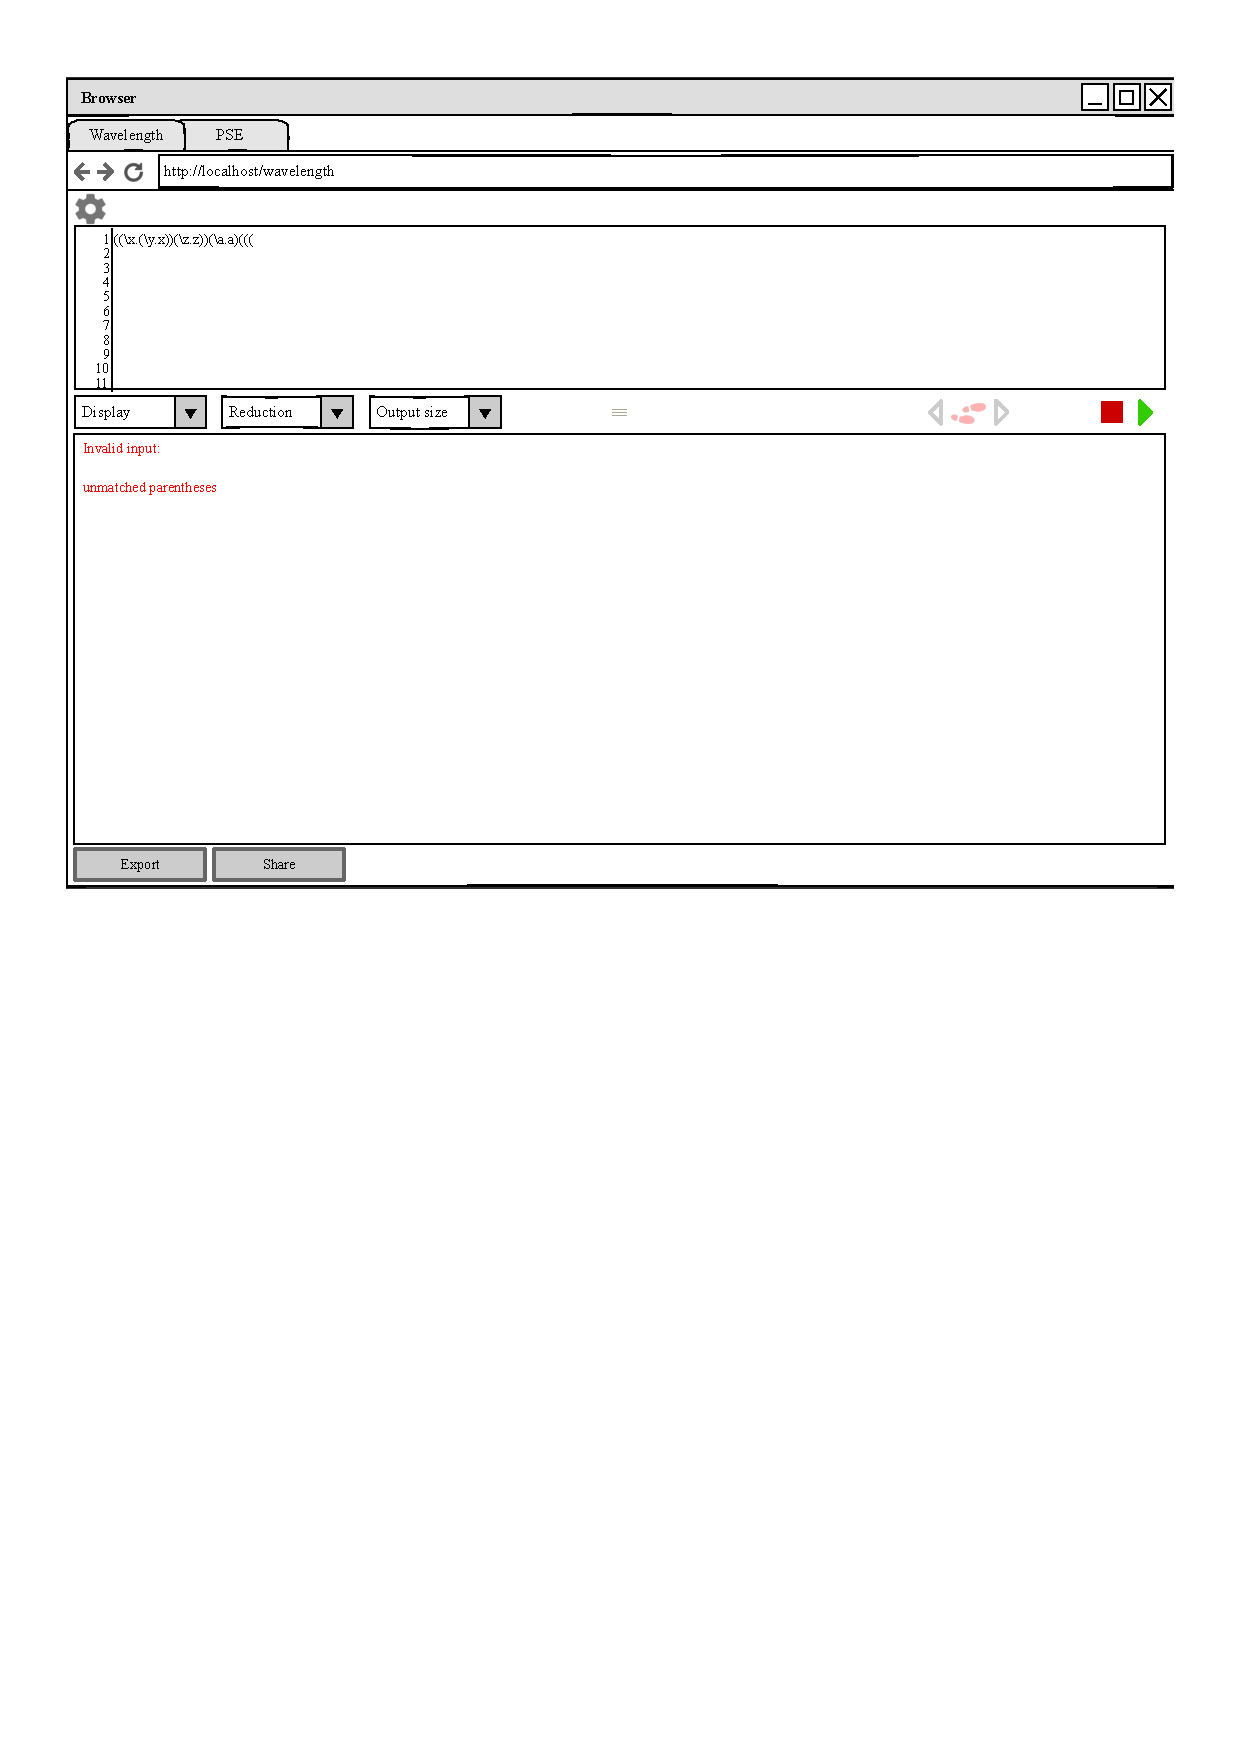
\includegraphics[width=\textwidth]{img/fehlerausgabe}
	\caption{Bei fehlerhafter Eingabe wird eine Fehlermeldung im Ausgabefeld ausgegeben.
}
\end{figure}



\begin{figure}[H]
	\begin{subfigure}{0.25\textwidth}
		\centering
		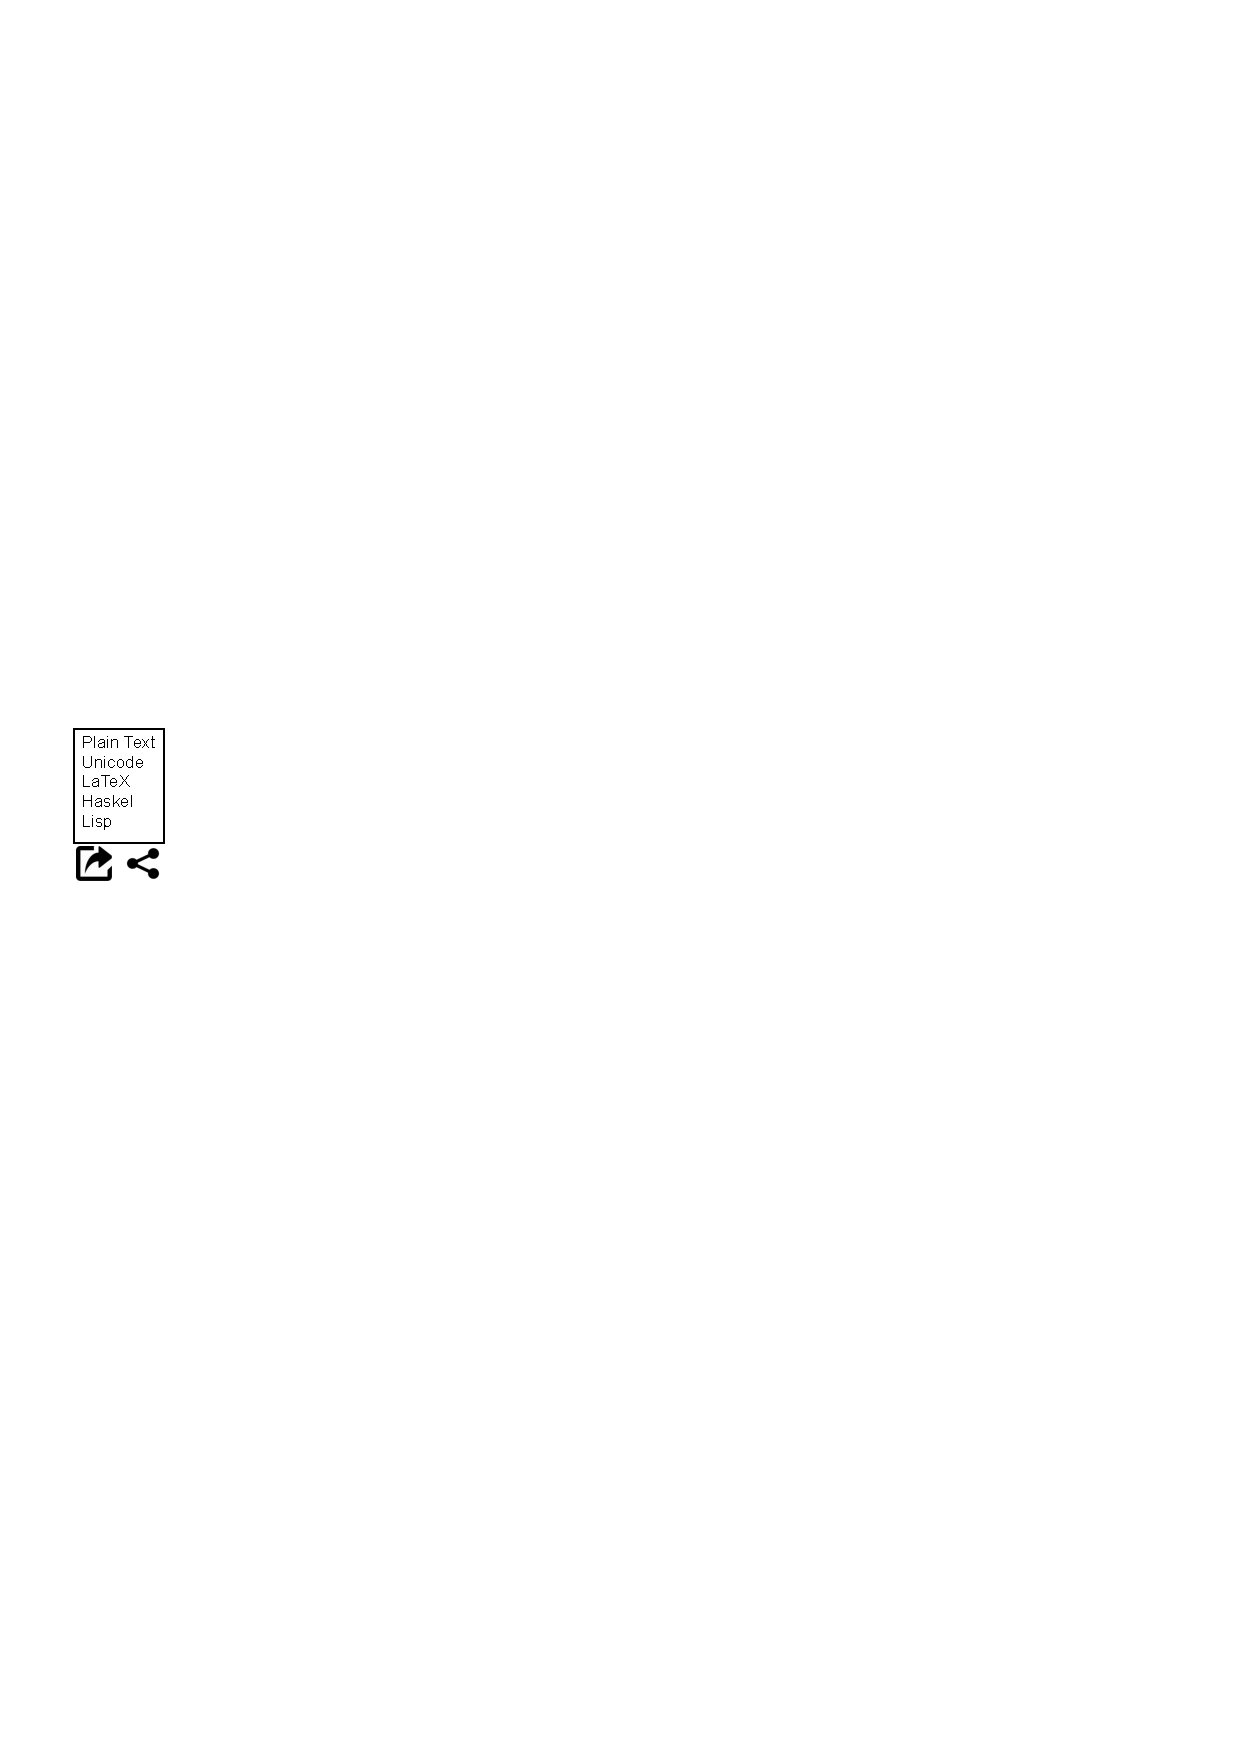
\includegraphics{img/exportMenu}
	\end{subfigure}
	\begin{subfigure}{0.75\textwidth}
		\centering
		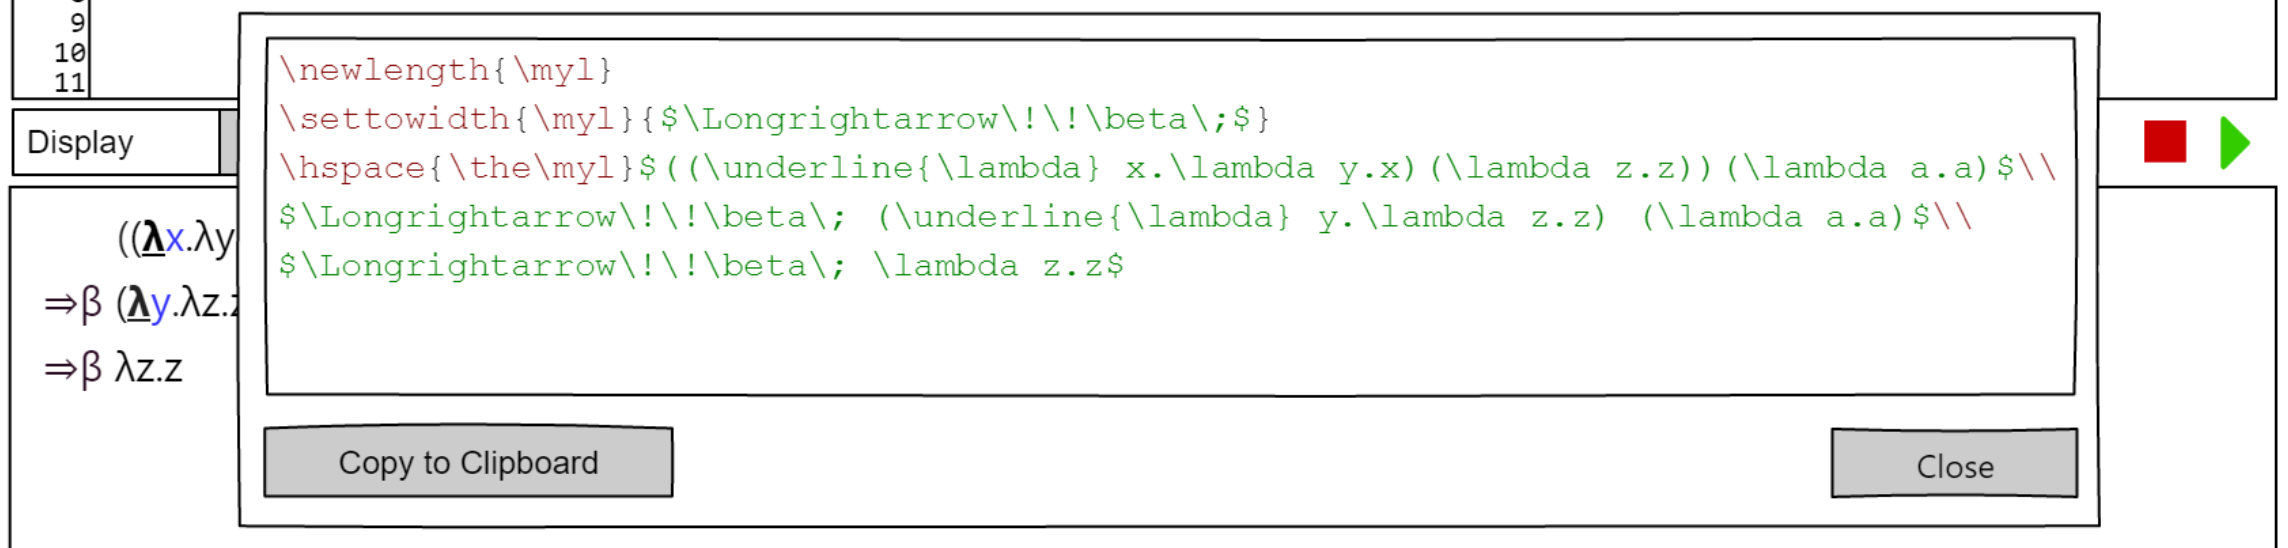
\includegraphics[width=1.1\textwidth]{img/export_latex_ausschnitt.png}
	\end{subfigure}
	\caption{\label{fig:export}Durch Klick auf den Export-Knopf kann der aktuelle Inhalt des Ausgabefelds in das gewünschte Format exportiert werden (Hier \LaTeX -Quellcode).}
\end{figure}


\begin{figure}[H]
	\centering
	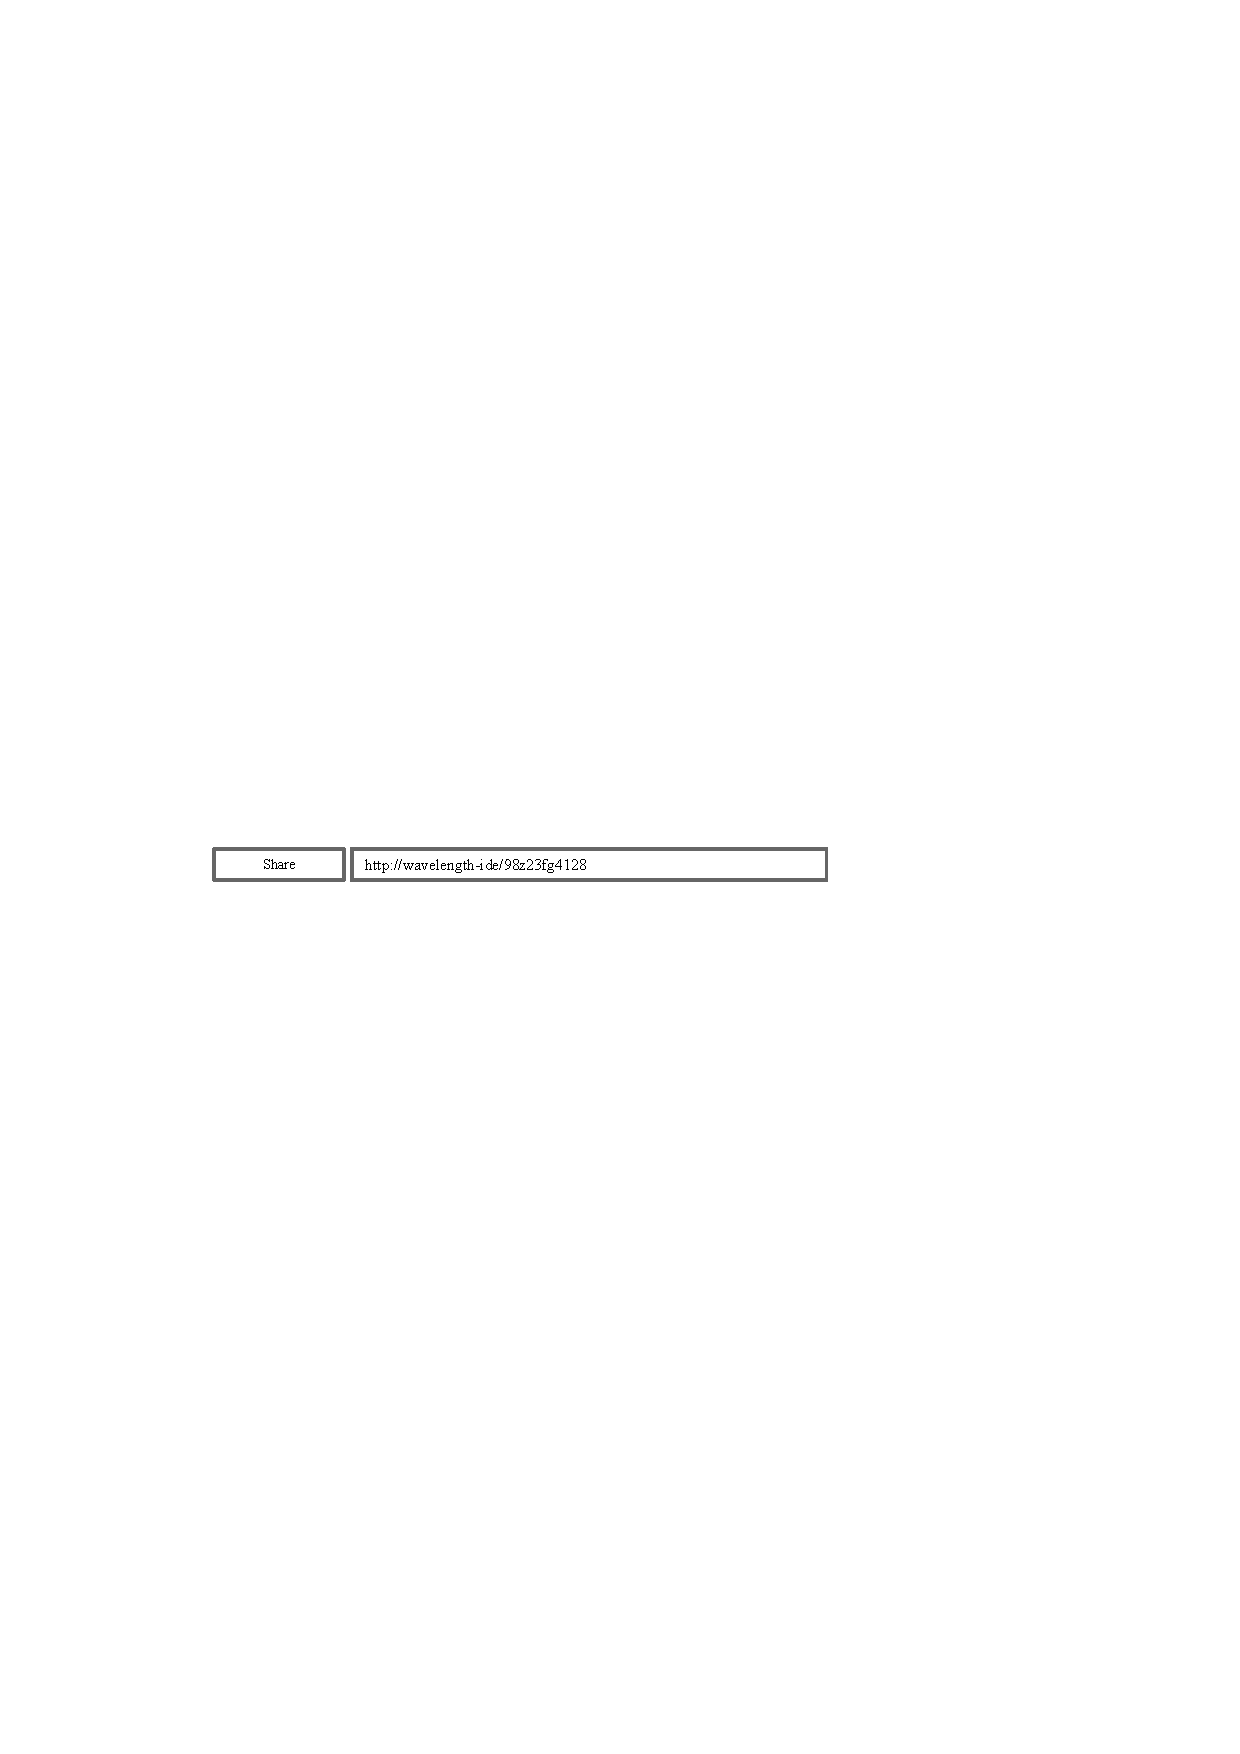
\includegraphics{img/share}
	\caption{Bei Betätigen des Teilen-Knopfes wird ein entsprechender Link erstellt.}
	\label{img:share}
\end{figure}


\begin{figure}[H]
	\centering
	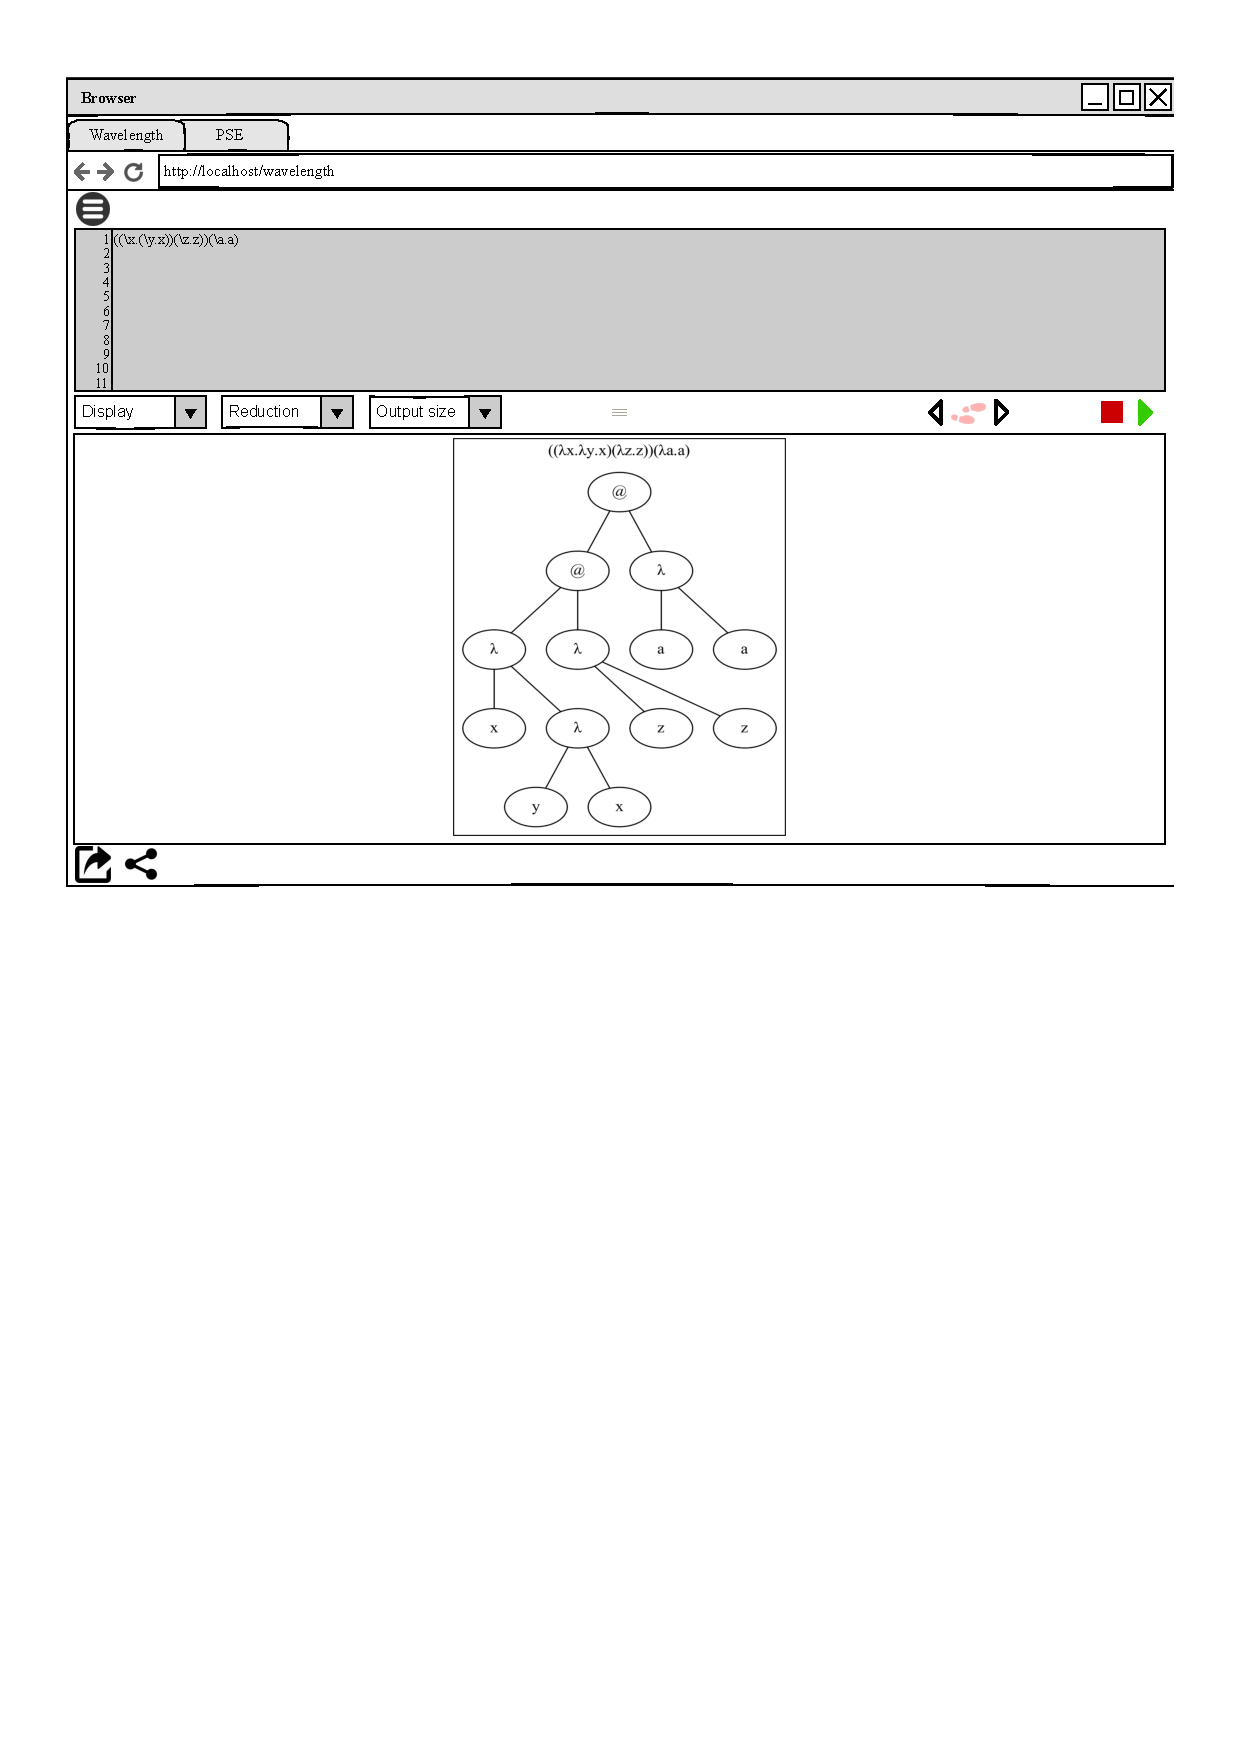
\includegraphics[width=\textwidth]{img/displayTree1}
	\caption{\label{fig:tree}Wird das Ausgabeformat "Tree" ausgewählt (siehe \cref{fig:outputOptions}), so werden einzelne Schritte der Ausführung als Syntaxbaum im Ausgabefeld angezeigt.}
\end{figure}


\begin{figure}[H]
	\begin{subfigure}{0.25\textwidth}
		\centering
		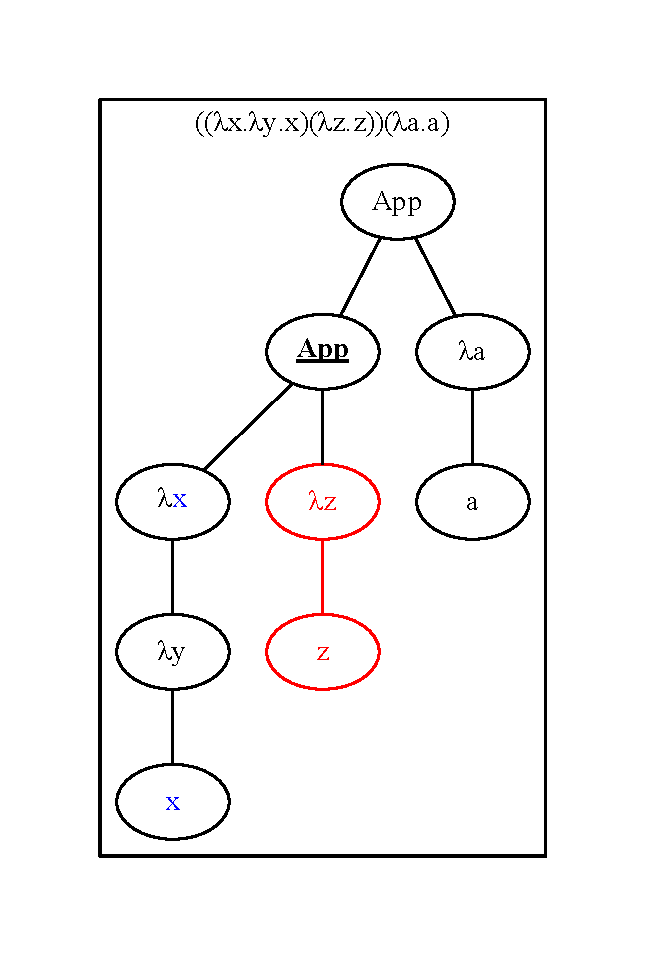
\includegraphics[width=\textwidth]{img/displayTree2}
		\caption{\label{fig:ltAppTreeA}Syntaxbaum mit ausgewählter \gls{lapp} (unterstrichen).}
	\end{subfigure}
	\hspace*{\fill}
	\begin{subfigure}{0.25\textwidth}
		\centering
		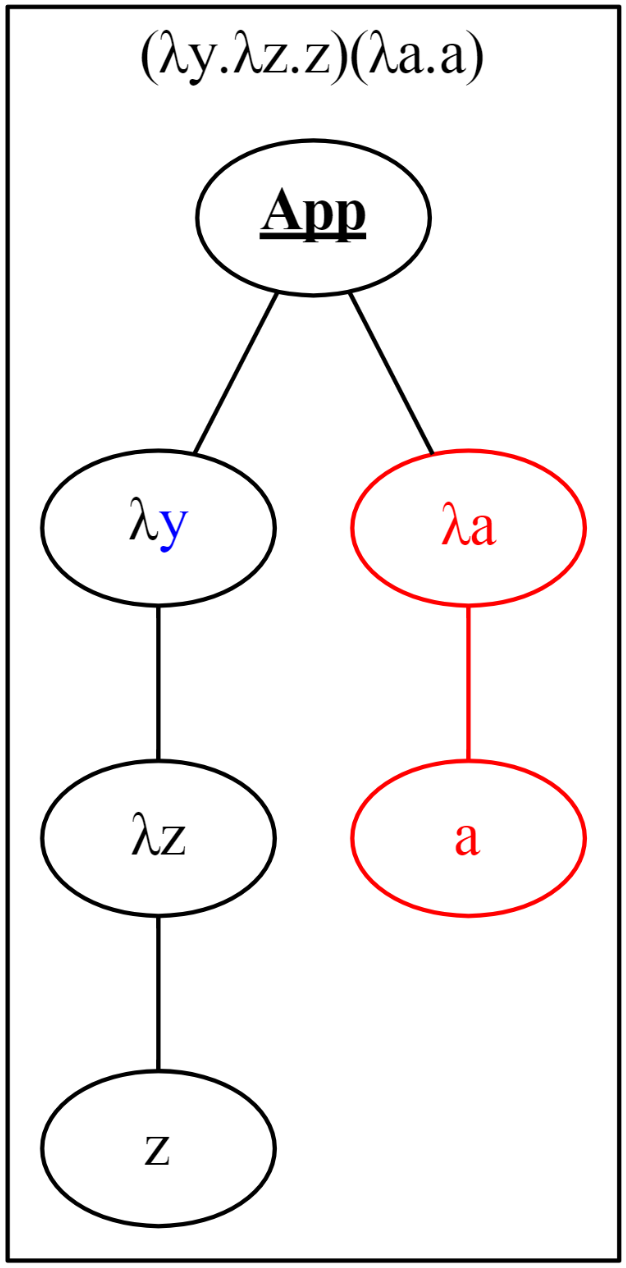
\includegraphics[width=0.85\textwidth]{img/displayTree6.png}
		\caption{\label{fig:ltAppTreeB}Neue Ausgabe beim Anklicken der ausgewählten \gls{lapp}.}
	\end{subfigure}
	\hspace*{\fill}
	\begin{subfigure}{0.25\textwidth}
		\centering
		
\includegraphics[width=\textwidth]{img/displayTree5}
		\caption{Endausgabe bei Auswahl der Wurzel.}	
	\end{subfigure}
	\caption{Wird ein "App"-Symbol (\gls{lapp}) angeklickt, so wird dieser Teilterm reduziert und der neue Syntaxbaum angezeigt.}
\end{figure}


\begin{figure}[H]
	\centering
	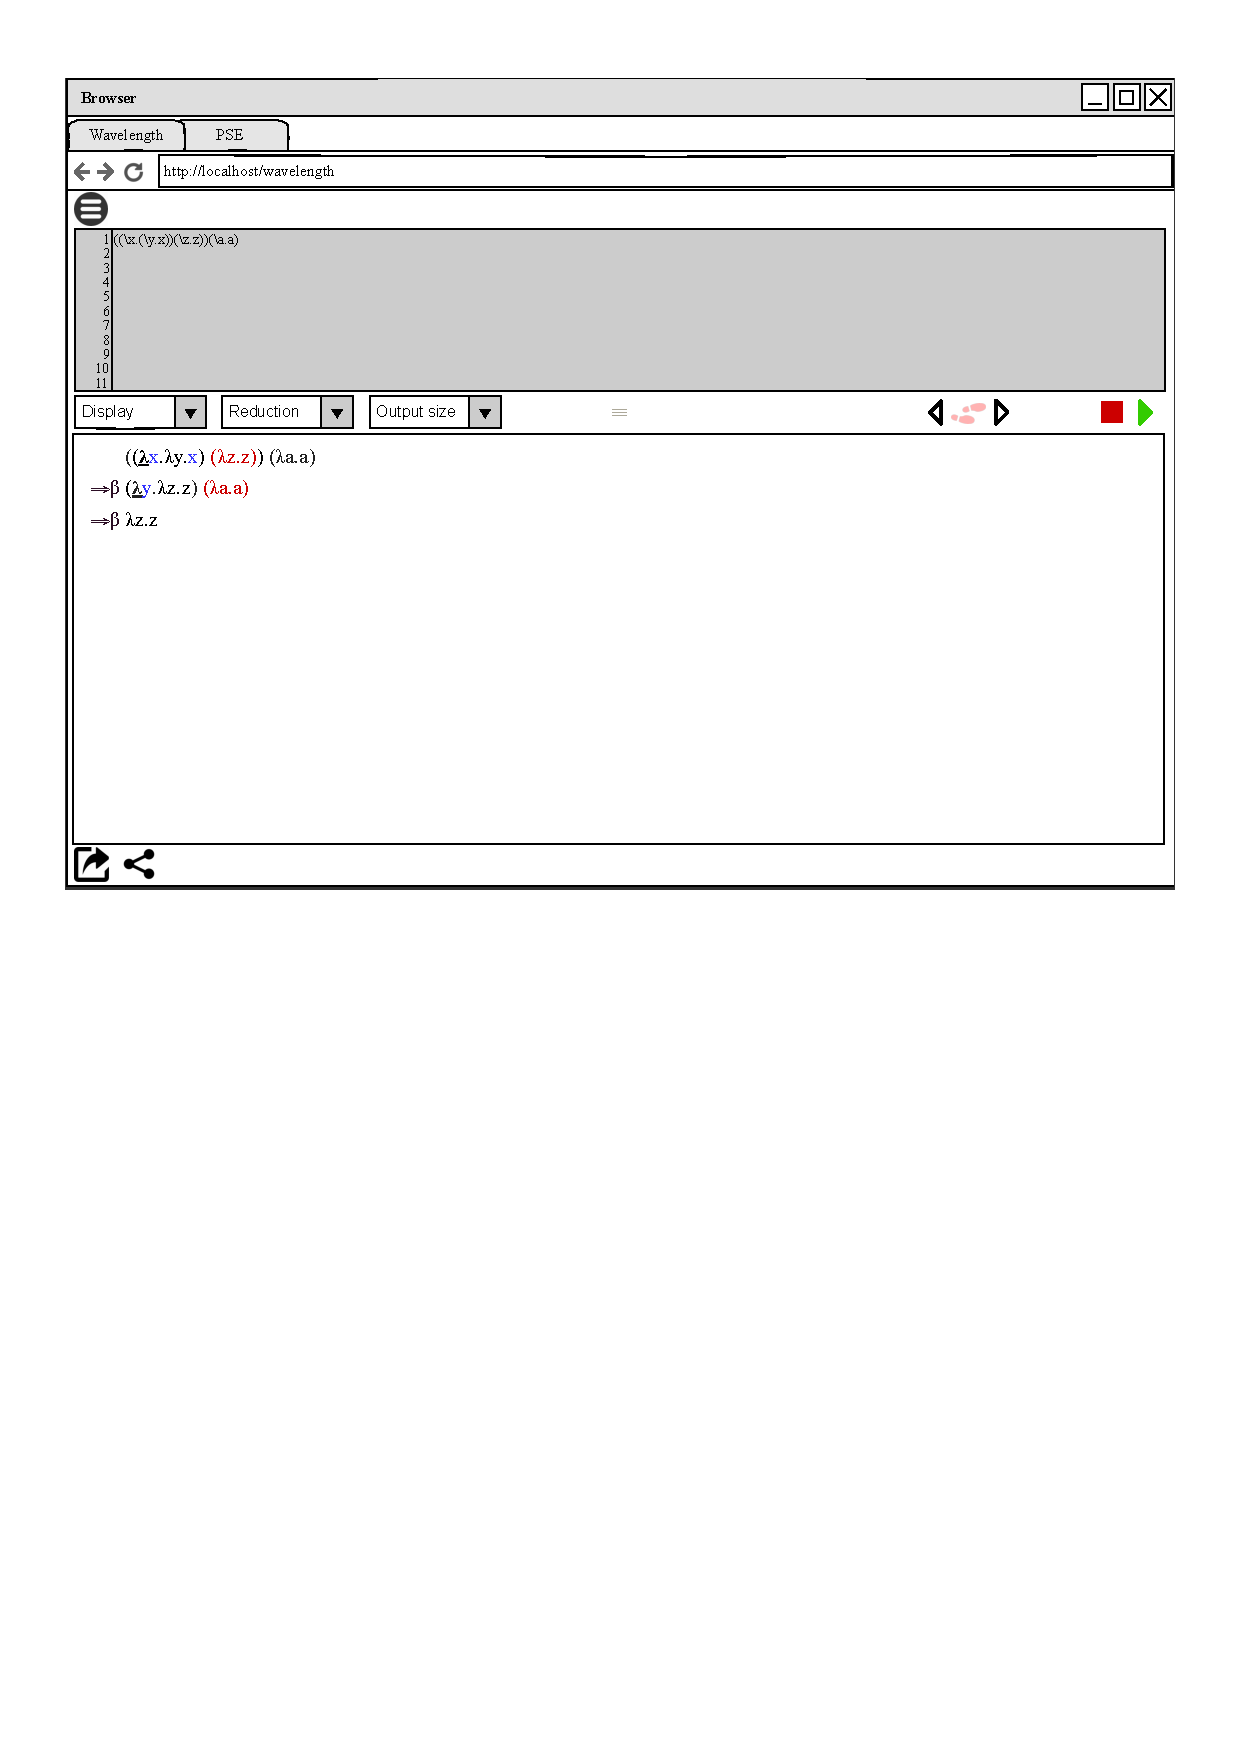
\includegraphics[width=\textwidth]{img/Unicode_Darstellunsgmodus}
	\caption{\label{fig:unicode}Wird das Ausgabeformat "Unicode" ausgewählt (siehe \cref{fig:outputOptions}), so wird der eingegebene \gls{lt} mit Unicode-$\lambda$-Zeichen im Ausgabefeld angezeigt.}
\end{figure}

\pagebreak

%%%%%%%%%
\section{Glossar}

\printglossaries

\end{document}
